%%% The main file. It contains definitions of basic parameters and includes all other parts.

%% Settings for single-side (simplex) printing
% Margins: left 40mm, right 25mm, top and bottom 25mm
% (but beware, LaTeX adds 1in implicitly)
\documentclass[12pt,a4paper]{report}
\setlength\textwidth{145mm}
\setlength\textheight{247mm}
\setlength\oddsidemargin{15mm}
\setlength\evensidemargin{15mm}
\setlength\topmargin{0mm}
\setlength\headsep{0mm}
\setlength\headheight{0mm}
% \openright makes the following text appear on a right-hand page
\let\openright=\clearpage

%% Settings for two-sided (duplex) printing
% \documentclass[12pt,a4paper,twoside,openright]{report}
% \setlength\textwidth{145mm}
% \setlength\textheight{247mm}
% \setlength\oddsidemargin{14.2mm}
% \setlength\evensidemargin{0mm}
% \setlength\topmargin{0mm}
% \setlength\headsep{0mm}
% \setlength\headheight{0mm}
% \let\openright=\cleardoublepage

%% Generate PDF/A-2u
%\usepackage[a-2u]{pdfx}

%% Character encoding: usually latin2, cp1250 or utf8:
\usepackage[utf8]{inputenc}

%% Prefer Latin Modern fonts
\usepackage{lmodern}

%% Further useful packages (included in most LaTeX distributions)
\usepackage{amsmath}        % extensions for typesetting of math
\usepackage{amsfonts}       % math fonts
\usepackage{amsthm}         % theorems, definitions, etc.
\usepackage{bbding}         % various symbols (squares, asterisks, scissors, ...)
\usepackage{bm}             % boldface symbols (\bm)
\usepackage{caption}
\usepackage{subcaption}

\usepackage{graphicx}       % embedding of pictures
\usepackage{fancyvrb}       % improved verbatim environment
\usepackage{natbib}         % citation style AUTHOR (YEAR), or AUTHOR [NUMBER]
\usepackage[nottoc]{tocbibind} % makes sure that bibliography and the lists
			    % of figures/tables are included in the table
			    % of contents
\usepackage{dcolumn}        % improved alignment of table columns
\usepackage{booktabs}       % improved horizontal lines in tables
\usepackage{paralist}       % improved enumerate and itemize
\usepackage[usenames]{xcolor}  % typesetting in color
\usepackage{hyperref}
\usepackage{pgfplots}
\usepackage{tikz}
\usepackage{algorithm}
\usepackage{algorithmic}
\usetikzlibrary{shapes,arrows,shadows,positioning,calc,fit}

%%% Basic information on the thesis

% Thesis title in English (exactly as in the formal assignment)
\def\ThesisTitle{Artificial Intelligence and Automated Reasoning}

% Author of the thesis
\def\ThesisAuthor{Martin Smolík}

% Year when the thesis is submitted
\def\YearSubmitted{2019}

% Name of the department or institute, where the work was officially assigned
% (according to the Organizational Structure of MFF UK in English,
% or a full name of a department outside MFF)
\def\Department{Department of Algebra}

% Is it a department (katedra), or an institute (ústav)?
\def\DeptType{Department}

% Thesis supervisor: name, surname and titles
\def\Supervisor{Mgr. Josef Urban, Ph.D.}

% Supervisor's department (again according to Organizational structure of MFF)
\def\SupervisorsDepartment{Department of Algebra}

% Study programme and specialization
\def\StudyProgramme{Mathematical structures}
\def\StudyBranch{study branch}

% An optional dedication: you can thank whomever you wish (your supervisor,
% consultant, a person who lent the software, etc.)
\def\Dedication{%
Dedication.
}

% Abstract (recommended length around 80-200 words; this is not a copy of your thesis assignment!)
\def\Abstract{%
In this thesis we aim to build algebraic models in computer using machine learning methods. We start with a set of axioms that describe functions and constants and use them to train neural networks approximating them. Every element is represented as a real vector, so that neural networks can operate on them. We also explore and compare different representations. Main focus in this thesis are groups. We build representations for cyclic (the simplest) and symmetric (the most complex) groups. Another part of this thesis is the aim to extend these built models by introducing new "algebraic" elements, not unlike the classic extension of rational numbers $\mathbb{Q}[\sqrt{2}]$. 
}

% 3 to 5 keywords (recommended), each enclosed in curly braces
\def\Keywords{%
{Machine learning} {Automated reasoning}  {Model theory} {Neural networks}
}

%% The hyperref package for clickable links in PDF and also for storing
%% metadata to PDF (including the table of contents).
%% Most settings are pre-set by the pdfx package.
\hypersetup{unicode}
\hypersetup{breaklinks=true}

% Definitions of macros (see description inside)
%%% This file contains definitions of various useful macros and environments %%%
%%% Please add more macros here instead of cluttering other files with them. %%%

%%% Minor tweaks of style

% These macros employ a little dirty trick to convince LaTeX to typeset
% chapter headings sanely, without lots of empty space above them.
% Feel free to ignore.
\makeatletter
\def\@makechapterhead#1{
  {\parindent \z@ \raggedright \normalfont
   \Huge\bfseries \thechapter. #1
   \par\nobreak
   \vskip 20\p@
}}
\def\@makeschapterhead#1{
  {\parindent \z@ \raggedright \normalfont
   \Huge\bfseries #1
   \par\nobreak
   \vskip 20\p@
}}
\makeatother

% This macro defines a chapter, which is not numbered, but is included
% in the table of contents.
\def\chapwithtoc#1{
\chapter*{#1}
\addcontentsline{toc}{chapter}{#1}
}

% Draw black "slugs" whenever a line overflows, so that we can spot it easily.
\overfullrule=1mm

%%% Macros for definitions, theorems, claims, examples, ... (requires amsthm package)

\theoremstyle{plain}
\newtheorem{thm}{Theorem}
\newtheorem{lemma}[thm]{Lemma}
\newtheorem{claim}[thm]{Claim}

\theoremstyle{plain}
\newtheorem{defn}{Definition}

\theoremstyle{remark}
\newtheorem*{cor}{Corollary}
\newtheorem*{rem}{Remark}
\newtheorem*{example}{Example}

%%% An environment for proofs

%%% FIXME %%% \newenvironment{proof}{
%%% FIXME %%%   \par\medskip\noindent
%%% FIXME %%%   \textit{Proof}.
%%% FIXME %%% }{
%%% FIXME %%% \newline
%%% FIXME %%% \rightline{$\square$}  % or \SquareCastShadowBottomRight from bbding package
%%% FIXME %%% }

%%% An environment for typesetting of program code and input/output
%%% of programs. (Requires the fancyvrb package -- fancy verbatim.)

\DefineVerbatimEnvironment{code}{Verbatim}{fontsize=\small, frame=single}

%%% The field of all real and natural numbers
\newcommand{\R}{\mathbb{R}}
\newcommand{\N}{\mathbb{N}}

%%% Useful operators for statistics and probability
\DeclareMathOperator{\pr}{\textsf{P}}
\DeclareMathOperator{\E}{\textsf{E}\,}
\DeclareMathOperator{\var}{\textrm{var}}
\DeclareMathOperator{\sd}{\textrm{sd}}

%%% Transposition of a vector/matrix
\newcommand{\T}[1]{#1^\top}

%%% Various math goodies
\newcommand{\goto}{\rightarrow}
\newcommand{\gotop}{\stackrel{P}{\longrightarrow}}
\newcommand{\maon}[1]{o(n^{#1})}
\newcommand{\abs}[1]{\left|{#1}\right|}
\newcommand{\dint}{\int_0^\tau\!\!\int_0^\tau}
\newcommand{\isqr}[1]{\frac{1}{\sqrt{#1}}}

%%% Various table goodies
\newcommand{\pulrad}[1]{\raisebox{1.5ex}[0pt]{#1}}
\newcommand{\mc}[1]{\multicolumn{1}{c}{#1}}


% Title page and various mandatory informational pages
\begin{document}
%%% Title page of the thesis and other mandatory pages

%%% Title page of the thesis

\pagestyle{empty}
\hypersetup{pageanchor=false}
\begin{center}

\centerline{\mbox{
\includegraphics[width=166mm]{../img/logo-en.pdf}}}

\vspace{-8mm}
\vfill

{\bf\Large MASTER THESIS}

\vfill

{\LARGE\ThesisAuthor}

\vspace{15mm}

{\LARGE\bfseries\ThesisTitle}

\vfill

\Department

\vfill

\begin{tabular}{rl}

Supervisor of the master thesis: & \Supervisor \\
\noalign{\vspace{2mm}}
Study programme: & \StudyProgramme \\
\noalign{\vspace{2mm}}
Study branch: & \StudyBranch \\
\end{tabular}

\vfill

% Zde doplňte rok
Prague \YearSubmitted

\end{center}

\newpage

%%% Here should be a bound sheet included -- a signed copy of the "master
%%% thesis assignment". This assignment is NOT a part of the electronic
%%% version of the thesis. DO NOT SCAN.

%%% A page with a solemn declaration to the master thesis

\openright
\hypersetup{pageanchor=true}
\pagestyle{plain}
\pagenumbering{roman}
\vglue 0pt plus 1fill

\noindent
I declare that I carried out this master thesis independently, and only with the cited
sources, literature and other professional sources.

\medskip\noindent
I understand that my work relates to the rights and obligations under the Act No.~121/2000 Sb.,
the Copyright Act, as amended, in particular the fact that the Charles
University has the right to conclude a license agreement on the use of this
work as a school work pursuant to Section 60 subsection 1 of the Copyright Act.

\vspace{10mm}

\hbox{\hbox to 0.5\hsize{%
In ........ date ............	% FIXME!
\hss}\hbox to 0.5\hsize{%
signature of the author
\hss}}

\vspace{20mm}
\newpage

%%% Dedication

\openright

\noindent
\Dedication

\newpage

%%% Mandatory information page of the thesis

\openright

\vbox to 0.5\vsize{
\setlength\parindent{0mm}
\setlength\parskip{5mm}

Title:
\ThesisTitle

Author:
\ThesisAuthor

\DeptType:
\Department

Supervisor:
\Supervisor, \SupervisorsDepartment

Abstract:
\Abstract

Keywords:
\Keywords

\vss}

\newpage

\openright
\pagestyle{plain}
\pagenumbering{arabic}
\setcounter{page}{1}


%%% A page with automatically generated table of contents of the master thesis

\tableofcontents

%%% Each chapter is kept in a separate file
\chapter*{Introduction}
\addcontentsline{toc}{chapter}{Introduction}
\label{intro}

In this thesis we propose and try to build a new tool for automated theorem proving. Theorem provers, that is algorithms that given a theory and a conjecture find a formal proof, mostly use syntactic rules to manipulate formulas. This approach is very different from how human mathematicians think about mathematics. When a human is working with a theory, they usually do so with some sort of mental images of the structures that satisfy it. We aim to build these models for automatic provers, thus giving them the ability to also leverage the semantic meaning of the given theory. These models could be used as an oracle that guesses validity of given sentences by trying whether or not they hold in the trained models.

Another crucial aspect of intuitive understanding of structures is the ability to naturally extend them. Most structures have extensions that can be called "algebraic", i.e. those that arise when we add solutions to an equation that has no solution in the structure itself. Best known examples are algebraic extensions of rings, for example using the equation $x^2-2=0$ in $\mathbb{Z}$ or $x^2+1=0$ in $\mathbb{R}$.

The structures that mathematicians work with, however, can be quite complex. So complex in fact, that handcrafting a model that the computer can work with gets quite challenging. That is why we rely on machine learning, namely the universal property of the neural networks - their ability to approximate any continuous function with arbitrary precision. Neural network learning, however, needs to work with differentiable functions, that do not exist in most structures. To enable their usage we choose a representation of the structure elements in $\mathbb{R}^n$, which we will call \textit{grounding}. Here we will use exclusively handpicked groundings that give us better insight into the performance of the model.\\

The main subject and the main contribution of this thesis is the description and testing of the network architecture (inspired by \cite{serafini}) that enables the networks approximating the structure functions to learn using the propositions that are true in the structures. The description of this architecture can be found in \Autoref{chapter:implementation}. Using with the framework Tensorflow (\cite{tf}) we have built neural models and extensions of groups, namely $\mathbb{Z}_n$ and $S_n$. Results of these experiments can be found in \Autoref{chapter:results}.

Another minor contribution is the proof that the algebraic extensions of groups are always possible (in \Autoref{section:groups}). It is very likely that this was proven before, but we were unable to locate any such proof, thus we present this proof as our own.
\chapter{Background}
In this section we will discuss the fundamentals of both model theory and neural networks. Since this thesis seeks to unify two vastly different fields of mathematics and computer science, understanding of both of them is essential. A reader acquainted with those fields should not find any surprises here.

%--------------------------------------------------------------

\section{Model theory}
Model theory is the area of mathematics that studies mathematical structures through the lens of mathematical logic.
\subsection{Basic definitions}
\label{section:basics}
Most of these definitions are paraphrased from \cite{model}.
\begin{defn} A \textbf{language} $\mathcal{L}$ is a set of function, constant and relation symbols with associated arities.
\end{defn}

\begin{defn} A \textbf{term} in the language $\mathcal{L}$ is a finite sequence of function and constant symbols from $\mathcal{L}$ and variables that is defined recursively:
	\begin{enumerate}
	\item A variable is a term.
	\item A constant is a term.
	\item If $f$ is $n$-ary function and $t_1, \dots t_n$ are terms then $f(t_1, \dots t_n)$ is also a term.
	\end{enumerate}
Only sequences that can be obtained using this constructions are terms.
\end{defn}

\begin{defn} A \textbf{Formula} in the language $\mathcal{L}$ is a finite sequence of any symbols in $\mathcal{L}$, logical operations ($\wedge, \vee, \neg, \rightarrow$) and the equality symbol $=$. It is also defined recursively:
	\begin{enumerate}
		\item If $t_1$ and $t_2$ are terms then $t_1=t_2$ is a formula.
		\item If $R$ is an n-ary relation symbol and $t_1, \dots t_n$ are terms then $R(t_1, \dots t_n)$ is a formula. 
		\item If $\varphi$ is a formula then $\neg\varphi$ is also a formula.
		\item If $\phi$ and $\psi$ are formulas, then $\varphi\wedge\psi$, $\varphi\vee\psi$ and $\varphi\rightarrow\psi$ are also formulas.
	\end{enumerate}
	The definition usually also includes the quantifiers $\exists$ and $\forall$. 
	\begin{enumerate}
		\item[5.] If $\varphi$ is a formula and $x$ is a variable that is not already used with a quantifier then $(\exists x)\varphi$ and $(\forall x)\varphi$ are formulas.
		
		$\forall$ is called the \textit{universal} and $\exists$ is called the \textit{existential} quantifier
	\end{enumerate}
Once again, only sequences obtained by this construction are formulas. All subsequences of a formula that are also formulas are called \textbf{subformulas}.
\end{defn}

\begin{defn} Given a formula $\varphi$, a \textbf{free variable} is a variable in $\varphi$ that is not used in a quantifier. A variable that is used in a quantifier is called \textbf{bound}. If $x_1,\dots x_n$ are all the free variables of $\varphi$ then we usually write $\varphi$ as $\varphi(x_1,\dots x_n)$ to show that it has free variables.  A \textbf{sentence} is a formula that has no free variables. A \textbf{free formula} is a formula that has only free variables.
\end{defn}

\begin{defn}An \textbf{$\mathcal{L}$-theory} is a set of sentences in the language $\mathcal{L}$.
\end{defn}

Note that theory can be also infinite. Also note that the cardinality of a theory of a finite language is at most countable\footnote{Assuming either countable set of variables, or taking the formulas "up to renaming of variables".}.

\begin{defn} A \textbf{structure} $\mathcal{S}$ is a collection $(S,\mathcal{I})$ where $S$ is a nonempty set (called the universe of $\mathcal{S}$) and $\mathcal{I}$ is an assignment that assigns interpretations to the elements of $\mathcal{L}$. Naturally it assigns function symbols to functions on $S$, constant symbols to elements of $S$ and relation symbols to relations on $S$ with their appropriate arities.
\end{defn}

Now we will need to know what does it mean for a sentence to be true in a structure. In order to do that we first need to know the values of terms.

\begin{defn}
Let $t(v_1\dots v_n)$ be an $\mathcal{L}$-term and $\phi:\{v_1,\dots v_n\}\longrightarrow S$ be an assignments of the variables to the universe of an $\mathcal{L}$-structure $\mathcal{S}$. Then we recursively assign values to subterms of $t$.
\begin{enumerate}
	\item Value of $v_i$ is $\phi(v_i)$
	\item Value of $c$ where $c$ is a constant is $\mathcal{I}(c)$
	\item If $t_1\dots t_m$ are terms with assigned values $s_1\dots s_m$ and $f$ is a function then $f(t_1,\dots t_m)$ is assigned the value $\mathcal{I}(f)(s_1,\dots s_m)$.
\end{enumerate}
\end{defn}

\begin{defn}
	Let $\varphi(x_1,\dots x_n)$ be an $\mathcal{L}$-formula and $\mathcal{S}$ an $\mathcal{L}$-structure. Then given a variable assignment $\phi:\{x_1,\dots x_n\}\longrightarrow S$ we assign the truth value of all subformulas of $\varphi$ as follows:
\begin{enumerate}
	\item If the subformula is of the form $t_1(x_1,\dots x_m)=t_2(x_1,\dots x_m)$ where $t_1$ and $t_2$ are terms, then it is true if and only if $t_1$ and $t_2$ have the same value assigned with variable assignment $\phi$.
	\item If the subformula is of the form $R(t_1, \dots t_r)$ where $t_1, \dots t_r$ are terms with assigned values $s_1, \dots s_r$ then it is true if and only if $\mathcal{I}(R)(s_1,\dots s_r)$ holds in $\mathcal{S}$.
	\item Any logical operators work as normal, e.g. $\neg \psi$ is true if and only if $\psi$ is false or $\psi_1 \wedge \psi_2$ is true if and only if both $\psi_1$ and $\psi_2$ are true in this assignment. 
	\item If the subformula is of the form $(\forall y) \psi(y,x_1,\dots x_m)$ then it is true if and only if for any extension $\phi'$ of $\phi$ that also assigns $y$ does $\psi(y,x_1,\dots x_m)$ hold (with assignment $\phi'$).
	
	Alternatively if the subformula is of the form $(\exists y)\psi(y,x_1,\dots x_m)$ then we only require that there exists at least one such $\phi'$.
\end{enumerate}
\end{defn}

\begin{defn}
Given an $\mathcal{L}$-formula $\varphi(x_1,\cdots x_n)$ we say that $\varphi$ \textbf{holds} in an $\mathcal{L}$-structure $\mathcal{S}$ if it is true for any variable assignment. This is denoted as $\mathcal{S}\models \varphi(x_1,\dots x_n)$. A formula $\varphi$ is \textbf{satisfiable} if there exists a structure $\mathcal{S}$ in the same language where $\mathcal{S}\models \varphi$
\end{defn}
Note that this definition also works if $\varphi$ is a sentence.

\begin{defn}
Given an $\mathcal{L}$-theory $T$, we say that an $\mathcal{L}$-structure $\mathcal{S}$ is a \textbf{model} of $T$ if $T\models \varphi$ for every $\varphi\in T$.
\end{defn}
This $\mathcal{S}$ is by no means unique. In fact, most theories have vastly different models.

\begin{defn}
Formulas $\varphi$ and $\psi$ are \textbf{equivalent} if they are both true under the same variable assignments of their free variables in any of their models\footnote{This definition is not the standard one, since we only define equivalence with respect to models. Normally equivalence of formulas is a semantic property, regardless of models or even satisfiability. However, to define equivalence properly, we would need to define multiple other terms from mathematical logic, which we will not do for better readability of this section. Classic definition can be found in \cite{logic}.}.
\end{defn}

Note that this definition does not include semantic differences, e.g. renaming of variables. For this we use a different definition:

\begin{defn}
	We say that $\mathcal{L}$-formulas $\varphi$ and $\psi$ are \textbf{equisatistfiable} if either both are satisfiable or both are not.
\end{defn}

The models of $\varphi$ and $\psi$ can be different, they might not even be in the same language. Every pair of equivalent formulas is also equisatisfiable, since they share all models \footnote{This is also true with the classical definition of equivalence, even though it does not require the formulas to be satisfiable.}. This term is used almost exclusively in formula manipulations.

Important things to notice in this section are that the universe $S$ has no restrictions. The models trained by us use $S$ as a subset of $\mathbb{R}^n$ in order to allow working with neural networks. 

\subsection{Skolemization}
\label{section:skolem}
Existential quantifiers have been a major hurdle for automatic theorem provers, since they add a lot of complexity to the proving algorithms. For example if a formula starts with $\forall x \exists y \forall z$ then $y$ can be completely different for each $x$, but does not depend on $z$. To "remember" this dependency in further proofs, the theorem prover needs to do some processing. We call this process \textbf{Skolemization} by its inventor, Thoralf Skolem.

\begin{defn}
	We say that a formula $\varphi$ is in \textbf{prenex normal form} if it is written as a sequence of quantifiers followed by a free formula.
\end{defn}

\begin{thm}
	Every formula is equivalent to a formula in prenex normal form.
\end{thm}
\begin{proof}
	We recursively apply the quantifier equivalence rules (we also assume that there exists at least one element):
	\begin{itemize}
		\item $(Q x\ \varphi)\wedge\psi$ is equivalent to $Q x\ (\varphi\wedge\psi)$ where $Q$ is either $\exists$ or $\forall$. 
		\item $(Q x\ \varphi)\vee\psi$ is equivalent to $Q x\ (\varphi\vee\psi)$ where $Q$ is either $\exists$ or $\forall$. 
		\item $\neg(\exists x\varphi)$ is equivalent to $\forall x \neg \varphi$
		\item $\neg(\forall x\varphi)$ is equivalent to $\exists x \neg \varphi$
	\end{itemize}
If we treat implication $\varphi \rightarrow \psi$ as equivalent to $\neg \varphi \vee \psi$ we are done.
\end{proof}

\begin{defn}
	We say that a formula $\varphi$ is in \textbf{Skolem normal form} if it is in prenex normal form and all quantifiers are universal.
\end{defn}

Skolemization is a process that turns formulas from prenex normal forms to Skolem normal form by introducing new function and constant symbols. We repeatedly apply this step:

Let $\varphi$ be a formula that has the form $$\forall x_1\forall x_2,\dots \forall x_{i}\exists y\psi(x_1,\dots x_i,y)$$ where $x_1,\dots x_n$ are all universally quantified and $\psi$ is a formula in prenex normal form. Then the Skolemized version of $\varphi$ is obtained by introducing a new $i$-ary function symbol $f_y$ and replacing all occurrences of $y$ in $\psi$ with $f_y(x_1,\dots,x_i)$. Thus we get $$\forall x_1\forall x_2,\dots \forall x_{i}\psi(x_1,\dots x_i,f_y(x_1,\dots,x_i))$$ We say that $f_y$ is the Skolem function of $y$.

If $\varphi$ has the form $\exists y \psi(y)$, i.e. there are no universal quantifiers at the start we introduce a Skolem constant $c_y$ and replace all occurrences of $y$ in $\psi$ by $c_y$, obtaining $\psi(c_y)$. This is consistent with the notion of constants being $0$-ary functions.

\begin{thm}
	Every formula $\varphi$ is equisatisfiable to the formula $\phi$ that is obtained by the Skolemization process.
\end{thm}
\begin{proof}
	We need to prove that we can build a model of $\phi$ from a model of $\varphi$ and vice versa. Let $\mathcal{S}$ be a model of $\varphi$ and WLOG let $\varphi$ be in prenex normal form $Q_1x_1,\dots Q_nx_n\psi(x_1,\dots x_n)$ where $Q$-s are quantifiers and $\psi$ is a free formula. We need to add interpretations of all Skolem functions and constants to build the model $\mathcal{S}'\models\phi$. 
	
First, let us assume that $y$ is the first existentially quantified variable in $\varphi$ and $f_y(x_1,\dots,x_i)$ its Skolem function (to include Skolem constants we permit $i=0$). Since $\mathcal{S}$ is a model of $\varphi$, we know that for every $x_1,\dots x_i\in S$ there exists an $y$ that is the "witness" that $\varphi$ holds. We define $f_y(x_1,\dots x_i)=y$. Since there is such $y$ for every tuple of $x$-es, this is a well-defined function. And we can easily see, $\psi(x_1,\dots x_i,y,x_{i+2},\dots x_n)$ has the same truth value in $\mathcal{S}$ as $\psi(x_1,\dots x_i,f_y(x_1,\dots x_i),x_{i+2},\dots x_n)$ does in $\mathcal{S}'$, therefore $\mathcal{S}'\models\phi$. We repeat this process of defining Skolem functions for every step of the Skolemization process, and we get the whole $\mathcal{S}'$.

The other way around is just as easy. Since $\psi(x_1,\dots x_i,f_y(x_1,\dots x_i), x_{i+1},\dots,x_n)$ holds in $\mathcal{S}'$, there obviously exists an $y\in S$ that $\psi(x_1,\dots x_i,y, x_{i+1},\dots,x_n)$, that being $y=f_y(x_1,\dots x_i)$.
\end{proof}

This process had first been introduced to prove a general theorem in model theory, but we will use it to enable manipulation with existential quantifiers. More about the usage of this theorem can be found in \cite{logic} and \cite{model}.

\subsection{Substructures and extensions}
\label{section:extensions}

In order to do any constructions in model theory, we need to know how models relate to each other. As it is right now, our models exist completely separately from each other, with the only comparisons being possible through the lens of formulas. However, if two structures are models of the same theory, we can not differentiate between them using just that theory. That is why we need the notions of substructures and extensions.

\begin{defn}
	Let $\mathcal{S},\mathcal{T}$ be structures in the same language $\mathcal{L}$. Then a \textbf{mapping} of $\mathcal{S}$ to $\mathcal{T}$ is any function $f:S\rightarrow T$ that satisfies the following (for any $x_1,..,x_n\in S$):
	\begin{enumerate}
		\item If $F$ is an $n$-ary function in $\mathcal{L}$ then $f(F_\mathcal{S}(x_1,\dots,x_n))=F_\mathcal{T}(f(x_1),\dots,f(x_n))$.
		\item If $c$ is a constant in $\mathcal{L}$ then $f(c_\mathcal{S})=c_\mathcal{T}$.
		\item If $R$ is an $n$-ary relation in $\mathcal{L}$ then $R_\mathcal{S}(x_1,\dots,x_n)$ holds if and only if $R_\mathcal{T}(f(x_1),\dots,f(x_n))$ holds.
	\end{enumerate}
If it also holds that $f$ is one-to-one, then $f$ is called an \textbf{embedding}.
\end{defn}

\begin{defn}
	We say that a structure $\mathcal{S}$ is a \textbf{substructure} of $\mathcal{S}'$ if they are in the same language, $S\subseteq S'$ and all symbol interpretations agree on $S$. That means that $(S,\left.\mathcal{I}\right|_S)$ is a structure. Here $\left.\mathcal{I}\right|_S$ means the assignments of symbols is the same but restricted to $S$.
	
	We also say that $\mathcal{S}'$ is an \textbf{extension} of $\mathcal{S}$
\end{defn}

There are not many things that hold in extensions for general. For example a carthesian product of two structures with naturally defined functions, constants and relations is an extension of both of them, but their elements do not necessarily "interact" with each other. To ensure this interaction we need new definitions.

\begin{defn}
	Let $\mathcal{S}$ be an $\mathcal{L}$-structure and $\mathcal{S}'$ its extension. Let $t_1(x)$ and $t_2(x)$ be $\mathcal{L}'$-terms with only one variable where $\mathcal{L}'$ is the language $\mathcal{L}$ with added names for each element of $S$. We say that the predicate\footnote{Predicate is a formula with only one free variable} $\varphi(x): "t_1(x)=t_2(x)"$ is an \textbf{equation} in $\mathcal{S}$. If $\varphi(x)$ holds for some $x\in S'$, we say that $x$ is the \textbf{solution} of $\varphi$. If the if $S$ is not a subset of the set of solutions of $\varphi$, we say that the equation is \textbf{non-zero}.
\end{defn}
\begin{defn}	
	Let $\mathcal{S}$ be a structure, $\mathcal{S}'$ its extension and let $s\in S'$ be an element. If there exists a non-zero equation $\varphi(x)$ in $\mathcal{S}$ for which $s$ is a solution then $s$ is \textbf{algebraic}\footnote{Normally we do not require the $\varphi$ to be an equation, but for the purposes of our model we will make this assumption}. If there is no such equation, then $s$ is \textbf{transcendental}.
\end{defn}

We see that every element $s\in S$ is algebraic. We can take $x=s$ as the equation.

A reader acquainted with field extensions will recognize these terms. Indeed, these are generalizations of those terms, so that the theory can be modified and applied to other structures than fields. A crucial difference is that this definition does not guarantee the existence of an extension. An example of this is $0\cdot x=1\cdot x$ in any field. However, there are classes of structures where every equation yields an algebraic extension. One such example are groups.

\subsection{Groups and their algebraic extensions}
\label{section:groups}

\begin{defn}
A \textbf{group} is a structure in the language $\{\cdot,^{-1},e\}$ (where $\cdot$ is binary function, $^{-1}$ is unary and $e$ is a constant) that also models the following theory\footnote{For the sake of simplicity we will use multiple $=$ signs in the definitions. To be absolutely correct, we could re-write these as $a=b=c \longrightarrow a=b\wedge b=c \wedge c=a$.}
\begin{enumerate}
	\item $\forall a,b,c\ (a\cdot b)\cdot c = a \cdot (b\cdot c)$
	\item $\forall a\ a\cdot e = e\cdot a = a$
	\item $\forall a\ a\cdot a^{-1}=a^{-1}a=e$
\end{enumerate}
We will call $\cdot$ \textbf{composition}, $^{-1}$ \textbf{inverse} and $e$ shall be \textbf{unit}.
\end{defn}

Note that this is the skolemized version of the theory that has $\exists e \forall a\ e\cdot a = a\cdot e = a$ or $\exists e(\forall a\ e\cdot a = a\cdot e = a \wedge\forall a \exists b\ a\cdot b = b\cdot a = e)$\footnote{Once again we use simplified notation.}. 

\begin{defn}
	A substructure of a group is a \textbf{subgroup} (denoted $G\leq G'$). We say that a subgroup is \textbf{normal} if $\forall x\in G'\ \forall g\in G\ x^{-1}\cdot g\cdot x\in G$, or simply $x^{-1}Gx\leq G$. We denote it as $G\trianglelefteq G'$.
\end{defn}

It can be proven that this subgroup is of the form $\{t(b_1,\dots b_n)|b_1,\dots b_n\in B, t \text{ is a term}\}$. It is also the intersection of all groups that contain $B$ (\cite{group}). Note that if we use this as a definition, we can expand the notion of a generated substructure to any model.

\begin{defn}
	Let $G$ be a group and $B$ a set of elements of $G$. Then a subgroup \textbf{generated} by $B$ is the smallest subgroup of $G$ that contains $B$. We denote it as $\langle B\rangle_G$.
\end{defn}

\begin{defn}
	Let $G\leq H$ be two groups. Then the sets $hG=\{h\cdot g|g\in G\}$ for any $ h\in H$ are called  \textbf{left cosets} of $G$. If $G$ is a normal subgroup, then we can induce a composition on these cosets: $hG\cdot h'G=(h\cdot h')G$ (a proof that this is really a group can be found in \cite{group}). We will call this group the \textbf{quotient group} $H/G$.
\end{defn}

As with algebraic extensions over fields, we can use this quotient group to craft an algebraic extension to any equation.

First, however, we need a group that we can do quotient of.

\begin{defn}
\label{freegroupdefn}
	Let $G$ be a group. Then we will define an extension $G[x]$ as such:
	\begin{itemize}
		\item Elements of $G[x]$ are formal strings of the form $g_1 x^{n_1}g_2 x^{n_2}\dots g_k x^{n_k}g_{k+1}$ where $k$ can be any integer (including $0$-in that case we have an element of $g$), $g_i$ are elements of $G$ (all except $g_1$ and $g_{k+1}$ have to be different from $e$) and $n_i$ are non-zero integers.
		\item $\cdot$ is defined as concatenation of strings with adjustment for inverses. We do this adjustment by repeating the following:
			\begin{enumerate}
				\item If we there is a substring $g_i g_{i+1}$ where $g_i$ and $g_{i+1}$ are elements of $G$, we replace it with their product in $G$: $(g_i\cdot g_{i+1})$.
				\item If there is a substring $x^{n_{i-1}}ex^{n_i}$ we replace it by $x^{n_{i-1}+n_i}$.
				\item If there is $x^0$, we replace it by $e$.			
			\end{enumerate}
			If none of these replacements is possible, we have a valid element.
	\item $e$ is the same as in $G$.
	\item If  $g=g_1 x^{n_1}g_2 x^{n_2}\dots g_k x^{n_k}g_{k+1}$ then $g^{-1}=g_{k+1}^{-1}x^{-n_k}\dots x^{-n_1}g_1^{-1}$. We can easily verify that $g\cdot g^{-1}$ is indeed equal to $e$.
	\end{itemize}
We will still treat $G$ as a subgroup of $G[x]$, by identifying all elements of $G$ with a string made up by just this element.
\end{defn}

Without loss of generality we can assume that any equation $\varphi$ has the form $t(x)=e$, where $t$ is a term. If $\varphi(x): "t_1(x)=t_2(x)"$ would have a different form, then $\varphi'(x): "t_1(x)\cdot (t_2(x))^{-1}=e"$ has exactly the same solutions. We can also assume that every term $t(x)$ is equivalent to an element of $G[x]$, because the simplifications described in Definition \Autoref{freegroupdefn} produce terms that are equivalent, i.e. they yield the same values under the same variable assignment.

\begin{defn}
	Let $t$ be an element of $G[x]$ of the form $g_1 x^{n_1}g_2 x^{n_2}\dots g_k x^{n_k}g_{k+1}$. The \textbf{degree} of $t$ is $\sum_{i=1}^k n_i$.
	
\end{defn} 

We also naturally assign degrees to terms. For every term $t(x)$ that corresponds to $t\in G[x]$, we say that degree of $t(x)$ is the degree of $t$ as defined above.

\begin{lemma}
\label{degreelemma}
	For any $t,t'\in G[x]$ with degrees $n,m$. the following hold:
	\begin{enumerate}
		\item $t\cdot t'$ has the degree $n+m$.
		\item $t^{-1}$ has the degree $-n$
	\end{enumerate}
\end{lemma}
\begin{proof}
	The part 2 is easily seen from the definitions of $^{-1}$ in $C[x]$ and the degree.
	
We observe that the adjustments described in Definition \autoref{freegroupdefn} do not change the sum of exponents of the $x$-es. Thus $t\cdot t'$ has the same degree as the sum of exponents of $x$-es in concatenation of strings $t$ and $t'$. This sum is obviously $n+m$.
\end{proof}

\begin{thm}
	Let $G$ be a group and $\varphi(x)$ an equation of the form $t(x)=e$ with a non-zero degree $d$. Then there exists an extension $G'$ of $G$ such that there exists $g\in G'$ that is a solution to $\varphi$.
\end{thm}
\begin{proof}
Without loss of generality we asume that $t(x)$ has the form $g_1 x^{n_1}g_2 x^{n_2}\dots g_k x^{n_k}g_{k+1}$. This modification of $\varphi$ still has the same solutions.

Let $t$ be an element of $G[x]$ corresponding to $t(x)$. Let us then define $B=\{ptp^{-1}|p\in G[x]\}$. $\langle B\rangle$ is a normal subgroup of $G[x]$. We immediately see that $pbp^{-1}\in \langle B\rangle$, (even $pbp^{-1}\in B$) for all $b\in B, p\in G[x]$. Now if $b=b_1 b_2\dots b_n$ where $b_i\in B$ then $$pbp^{-1}=pb_1 b_2\dots b_np^{-1}=pb_1p^{-1}p b_2p^{-1}\dots pb_np^{-1}.$$
We define ${b_i}'=pb_ip^{-1}$ for $i\in\{1,\dots,n\}$. Now $$pbp^{-1}=(pb_1p^{-1})(p b_2p^{-1})\dots (pb_np^{-1})={b_1}'{b_2}'\dots{b_n}'.$$
Since $\forall i\ {b_i}'\in B$, also $pbp^{-1}\in \langle B\rangle$ and thus $\langle B \rangle$ is normal.

Also note that by Lemma \Autoref{degreelemma} all elements of $B$ have degree $d$. Thus no elements of $G[x]$ that have degree 0 are in $B$. Therefore every element of $B$ contains at least one occurrence of $x^n$ (where $n\neq 0$). 

Since $\langle B \rangle$ is a normal subgroup of $G[x]$, we know that $G[x]/\langle B \rangle$ is a group. In it, all the elements of $G$ form different cosets, since $g\langle B \rangle$ always has the element $g\cdot t$ and no two $g\in G$ can produce the same $g\cdot t$. Assuming that $g\notin \langle B \rangle\ \forall e\neq g\in G$, $G$ is isomorphic to a subgroup of $G[x]/\langle B \rangle$, and thus it can be seen as an extension of $G$.

Next we need to show is that $x \langle B \rangle$ is a solution to $\varphi(x)$. Indeed, since $t\in\langle B \rangle$, $$t(x\langle B \rangle)=t(x)\langle B \rangle=\langle B \rangle=e_{G[x]/\langle B \rangle}.$$

Therefore $G[x]/\langle B \rangle$ is the desired extension.

Lastly, we need to prove that $g\notin \langle B \rangle\ \forall g\in G, g\neq e$. Let $g$ be a counterexample, meaning that $g=\beta_1\beta_2\dots \beta_n$ where $\forall i$ either $\beta_i\in B$ or $\beta_i^{-1}\in B$. We can assume that $\beta_1$ starts with $g$ and $\beta_k$ ends with $e$ (or rather, a power of $x$). That is because if $\beta_1$ starts with $k$ and $\beta_2$ ends with $l$, where $kl=g$ in $G$ (the only possibility of obtaining $g$ is if all occurences of $x$ annihilate each other), we take $\beta'_i$ to be $l\beta_il^{-1}$ and we get the desired start. Then $\beta_1$ ends with $g^{-1}$. $\beta_2$ therefore has to start with $g$. By inducdtion we see that $\forall i \beta_i$ has to start with $g$ and end with $g^{-1}$. This is a contradiction with $\beta_k$ ending with a power of $x$.
\end{proof}

A reader acquainted with field extensions will probably recognize this construction. Indeed, it had been the inspiration for this proof.

The main difference, however, is that the extensions are not automatically unique, i.e. the groups that we can consider to be algebraic extensions are not necessarily isomorphic to each other. The property that ensures the uniqueness in field extensions is commutativity. We will show that commutative groups have unique comutative extensions.

\begin{defn}
	We say that a group is \textbf{commutative}, or \textbf{Abelian} if $a\cdot b = b \cdot a$ for any $a,b$.
\end{defn}

\begin{thm}
\label{theorem:abelian uniqueness}
	Let $G$ be a commutative group and $\varphi:t(x)=e$ an equation. Then there exists a commutative extension $G'$ of $G$ for which the following hold:
	\begin{enumerate}
	\item $G'$ contains a solution for $\varphi$
	\item If $H$ is a commutative extension of $G$ that contains a solution for $\varphi$, then $G'$ is isomporphic to a subgroup of $H$.
\end{enumerate}	 
\end{thm}
\begin{proof}
	We can redefine $G[x]$ to also be commutative (denoted $G_A[x]$), by adding a fourth inverse adjustment rule: replace $gx^n$ with $x^ng$. With this rule in place, we can see that all elements of $G_A[x]$ have the form $x^ng$ where $n\in\mathbb{Z},g\in G$.
	
	We can see that if we assume commutativity in $t(x)$, it is also equivalent (in the same sense as above) to an element $t\in G_A[x]$. 
	
	Therefore we may without loss of generality assume that $t(x)$ has the form $x^nc$. 
	
	If we construct $B=\{ptp^{-1}|p\in G_A[x]\}$ as above, we observe that due to commutativity it is just $\{t\}$. Therefore $\langle B\rangle=\{t^k|k\in \mathbb{Z}\}$. We once again construct $G_A[x]/\langle B\rangle$ that has the solution for $\varphi$ and is an extension of $G$. Any factor of a commutative group is commutative (\cite{group}). This group will be denoted $G'$.
	
	Let us explore the structure of $G'$. For the sake of simplicity we will denote the elements as $x^kg$.\footnote{Rather than the factor sets} We know that $x^n\cdot c=e$ in $G'$. Therefore $x^{-1}=x^{n-1}c$. Also, if $k>n$, then $x^kg=x^{k-n}c^{-1}g$. Therefore we can assume that for any element $x^kg$ it holds that $0\leq k<n$ (because every factor set has exactly one element of this form). 
	
	Now we shall prove the uniqueness of $G'$. Let $H$ be a commutative extension of $G$ that has an element $h$ that solves $\varphi$. Then $h^{-1}=h^{n-1}c$, since $h^nc=e$, just as well as $h^n=c^{-1}$. Therefore any element in this subgroup has the form $h^kg$ where $0\leq k<n$ and $g\in G$. We can easily see that this subgroup is isomorphic to $C'$ described above.
\end{proof}

These are however not the only extensions of commutative groups. The general construction only produces infinite non-commutative groups, since they will always contain infinite number of elements of the form $xgxgxg...xg$ (assuming $t$ has not the same form for the same $g$). 

%-------------------------------------------------------
%-------------------------------------------------------
%-------------------------------------------------------
%-------------------------------------------------------

\section{Neural networks}
Neural networks have been one of the most important and well developed methods in machine learning in recent years. The main advantage of their usage is their universal property - the fact that given an $\epsilon>0$ for every smooth function there exists  a neural network that approximates it with the error of at most $\epsilon$. Assuming that we have a structure whose universe is a subset of $\mathbb{R}^n$, we can approximate any of its functions with arbitrary precision\footnote{Assuming a suitable extension of the functions to facilitate the smoothness.}. How exactly do we do that will be discussed in \Autoref{chapter:implementation}. This section will introduce the reader to the basics of neural networks. More about this subject can be found in \cite{neural}. This publication is also the principal source for this section.

\subsection{What is a neural network}
\label{section:nn}
In this section we will describe a \textbf{feedforward neural network}. We call it feedforward because it lacks feedback connections. It is therefore simpler, although it does not have any "memory". If a network has feedback connections, it is called \textbf{recurrent}. Such networks are also widely used in machine learning, however they are not used here, and are beyond the scope of this thesis.

A network is a type of a smooth $\mathbb{R}^n\rightarrow\mathbb{R}^m$ function that has the form $f(x)=f_n(f_{n-1}(\dots f_1(\textbf{x}))\dots)$, where $f_i$ are real vector functions, called \textbf{layers}. We call $f_1$ the first layer, $f_2$ second and so on. The number of these layers is called the \textbf{depth} of a model. The last layer is called \textbf{output layer}, while the rest are called \textbf{hidden layers} since we usually can not interpret the meaning of the data used and produced by them.

In general the output of $f_i$ does not need to have the same dimension as the input $\textbf{x}$ or the output $\textbf{y}$. But for the sake of simplicity, all hidden layers usually tend to have the same dimension between them. This is called the \textbf{width} of the network. Both depth and width can have a profound effect on the network's performance. 

There is no overarching definition describing which functions are layers, thus every type of network may have a different type of layer function. However, in neural networks, there we almost always use a certain type of the layer function, which will describe here.

These layer functions consist of an affine transformation weight matrix $\textbf{W}$, bias vector $\textbf{b}$ and some activation function $\varphi:\mathbb{R}\rightarrow\mathbb{R}$. They are combined as $$f_i(\textbf{x})=\varphi\odot(\textbf{W}\textbf{x}+\textbf{b})$$ where $\varphi\odot (v_1,...,v_n)^\top$ denotes $(\varphi(v_1),...\varphi(v_n))^\top$, the element-wise application of $\varphi$. Activation functions and our requirements for them are further discussed below. 

The networks using this type of layers are called neural, because they are inspired by biological neurons. \Autoref{nndiagram1} illustrates the \textit{informal} intuition behind this. Each arrow represents a $\mathbb{R}\rightarrow \mathbb{R}$ function between two nodes. Each node represents a neuron that either "activates" or not, based on the sum of the functions leading to it and the activation function. The biological inspiration comes from the fact that biological neurons also either send a signal or not, based on the signals from surrounding neurons.

\begin{figure}[h]
\center
\caption{Neurons in a layer}
\label{nndiagram1}
\medskip
\begin{tikzpicture}[circ/.style={circle,draw,minimum size=1em}]
\foreach \i in {4,...,1}
{
	\node[circ](a\i)at(-1,\i){};
	\node[circ](b\i)at(1,\i){};
}
\foreach \i in {1,...,4}
{
	\draw[->,-latex'](a\i)--(b4);
	\draw[->,-latex'](a\i)--(b3);
}
\end{tikzpicture}
\end{figure}	

The simplest neural networks are linear models, e.g. linear regression. In these models there is no activation function. These models are simple, however they have many drawbacks. The main one is their ability to only model linear functions. Indeed, if the layers are linear functions, several layers in a sequence also form a linear function.

We overcome this by introducing non-linearities via the activation functions. Activation function therefore has to be a \textit{non-linear} $\mathbb{R}\rightarrow \mathbb{R}$ function. We generally also require some degree of smoothness to enable optimalisation (see \Autoref{section:learning+opt}). There are several functions that fulfill this purpose, each with their advantages and disadvantages. The simplest is $ReLU$: the \textbf{Re}ctified \textbf{L}inear \textbf{U}nit (\cite{relu1}, \cite{relu2}, \cite{relu3}). It is defined as $ReLU(x)=max\{x,0\}$. It is the most used activation function because it is the simplest non-linear function that also preserves most of what makes linear functions easy to work with (simple derivation). It has however some drawbacks that we will discuss later, along with other used alternatives.

\begin{figure}[h]
\caption{ReLU}
\center
\begin{tikzpicture}
	\draw[->](-3,0)--(3,0)node[midway,anchor=north]{$0$}node[below left]{$x$};
	\draw[->](-3,0)--(-3,5)node[below left]{$y$};
	\draw[dotted](0,0)--(0,1);
	\node[anchor=east] at (-3,1){$0$};
	\draw[line width=2] (-3,1)--(0,1)--(3,4);
\end{tikzpicture}
\end{figure}

\subsection{Example: XOR}
\label{section:xor}
One of the simplest examples of the usefulness of this non-linearity is the binary operation XOR: the e\textbf{X}clusive \textbf{OR}. It is a function $\{0,1\}^2\rightarrow \{0,1\}$ that is $1$ if and only if exactly one of the inputs is $1$. This function is impossible to approximate with linear regression, but there exists a simple network with $ReLU$ activation functions that exactly approximates it. This example network is the same as can be found in \cite{neural}.

Let us start with linear regression. A linear regression model of a function $f:\mathbb{R}^n\rightarrow \mathbb{R}$ is a function $\widehat{f}_\theta$ that is affine, i.e. it inputs a vector $\textbf{x}=(x_1,...,x_n)$ and outputs a scalar $a_1x_1+...+a_nx_n+b$ where $\{a_1,...,a_n,b\}=\theta$ are some real parameters. The points $(x_1,...x_n,\widehat{f}_\theta(\textbf{x}))$ form an affine plane in $\mathbb{R}^{n+1}$. A plane of a linear regression model approximating XOR needs to intersect points $(0,0,0);(1,0,1);(0,1,1)$ and $(1,1,0)$. The only plane that intersects the first three is defined by the equation $x_1+x_2-y=0$. However, this does not intersect the last point.

Linear regression is usually optimized using the least squares method. This means that the parameters $\theta=\{a_1,...,a_n,b\}$ are defined as $$\theta=\text{argmin}_\theta\left\{\sum_{i=1}^k \left(f(\textbf{x}^{(i)})-\widehat{f}_\theta(\textbf{x}^{(i)})\right)^2\right\}$$ where $\{\textbf{x}^{(i)}\}_{i=1}^k$ is a finite set of points that we seek to approximate $f$ on. Using this method on our 4 points, the linear regression model of XOR function has parameters $a_1=a_2=0$ and $b=\frac{1}{2}$. This is a constant function $\widehat{f}(\textbf{x})=\frac{1}{2}$, an obviously unsatisfactory approximation.

If we however permit the usage of activation functions (ReLU), we can handcraft a network that will fit the function perfectly. Now our network will have the form 
$$\widehat{f}(\textbf{x};\textbf{W},\textbf{c},\textbf{w},b)=\textbf{w}^\top \max\{0,\textbf{W}^\top\textbf{x}+\textbf{c}\}$$ 
where 
$$\textbf{W}=
\left(\begin{matrix}
	1 & 1\\
	1 & 1
\end{matrix}\right),$$
$$\textbf{c}=
\left(\begin{matrix}
	0\\
	-1
\end{matrix}\right),$$
and
$$\textbf{w}=
\left(\begin{matrix}
	1\\
	-2
\end{matrix}\right).$$ This network is illustrated in \Autoref{xordiagram}. This is also not the only network that estimates XOR perfectly.
\begin{figure}[h]
\caption{XOR network}
\center
\label{xordiagram}
\begin{tikzpicture}
	\node[circle,draw](in1) at (0,0){$x_1$};
	\node[circle,draw](in2) at (2,0){$x_2$};
	\node[circle,draw](mid1) at (0,1.5){$\ \ \ $};
	\node[rectangle,draw](relu1) at (0,3){\small{ReLU}}; 
	\node[circle,draw](mid2) at (2,1.5){$\ \ \ $};
	\node[rectangle,draw](relu2) at (2,3){\small{ReLU}}; 
	\node[circle,draw](out) at (1,4.5){$y$};
	\draw[-latex](in1)--(mid1) node[pos=0.2,anchor=east]{$\cdot 1$};
	\draw[-latex](in1)--(mid2) node[pos=0.14,anchor=west]{$\cdot 1$};
	\draw[-latex](in2)--(mid1) node[pos=0.14,anchor=east]{$\cdot 1$};
	\draw[-latex](in2)--(mid2) node[pos=0.2,anchor=west]{$\cdot 1$};
	\draw[-latex](mid1)--(relu1) node[midway,anchor=east]{$+0$};
	\draw[-latex](mid2)--(relu2) node[midway,anchor=west]{$-1$};
	\draw[-latex](relu1)--(out) node[midway,anchor=east]{$\cdot 1$};
	\draw[-latex](relu2)--(out) node[midway,anchor=west]{$\cdot (-2)$};
	
\end{tikzpicture}
\end{figure}

Let us see what happens when we input the points in matrix form $$
\left(\begin{matrix}
	0 & 0\\
	1 & 0\\
	0 & 1\\
	1 & 1
\end{matrix}\right).$$
After the first layer multiplication by the weight matrix $\textbf{W}$ we have
$$\left(\begin{matrix}
	0 & 0\\
	1 & 1\\
	1 & 1\\
	2 & 2
\end{matrix}\right).$$

When we add the bias vector $\textbf{c}$ we get 
$$
\left(\begin{matrix}
	0 & -1\\
	1 & 0\\
	1 & 0\\
	2 & 1
\end{matrix}\right).$$

Now we apply ReLU:
$$
\left(\begin{matrix}
	0 & 0\\
	1 & 0\\
	1 & 0\\
	2 & 1
\end{matrix}\right).$$

This concludes the first layer of the network. Then we multiply each row with $\textbf{w}^\top$ and we get
$$	
\left(\begin{matrix}
	0\\
	1\\
	1\\
	0
\end{matrix}\right)$$
which is exactly the desired output.

In this case we got the hand-crafted solution from a book. Normally the weights and biases are found using an optimization method such as gradient descent (more about optimization can be found in \Autoref{section:learning+opt}). Here we found the perfect solution, a global minimum to the loss function. However that is not generally possible.

\subsection{Other activation functions}
\label{section:activation_functions}
ReLU, while being the most popular activation function, is not the one used in the models built for this thesis, because it also has some drawbacks. The fact that its gradient is $0$ on all negative inputs means that the optimization process may lead to the state where a node "dies" - all gradients regardless of data are 0. This tends to happen if our input and output contain few non-zero elements. In that case it is therefore advised to use a different activation function.

Before the introduction of ReLU the default activation functions were sigmoid $$\sigma(x)=\frac{1}{1+e^{-x}}$$ and hyperbolic tangent $$\tanh(x)=\frac{e^x-e^{-x}}{e^x+e^{-x}}$$ functions. They are related to each other since $\tanh(x)=2\sigma(2x)-1$. The main advantage of these functions is that they only output values in an open interval, $(0,1)$ for sigmoid and $(-1,1)$ for tanh. They also have nonzero gradient over their whole domain, which ensures that gradient descent optimization always works. However, as can be seen in \Autoref{sigmoiddiagram} if the inputs are far enough from $0$, the gradients become very small. This results in gradient descent optimizers taking longer time (\cite{imagenet_relu}). If this happens, we say that the functions \textbf{saturate}. This is also the reason why these functions largely fell out of use.
\begin{figure}[t]
\caption{Sigmoid and tanh functions}
\center
\label{sigmoiddiagram}
\begin{tikzpicture}
    \begin{axis}[
    	legend pos=north west,
        axis x line=middle,
        axis y line=middle,
        x tick label style={/pgf/number format/fixed,
                            /pgf/number format/fixed zerofill,
                            /pgf/number format/precision=1},
        y tick label style={/pgf/number format/fixed,
                            /pgf/number format/fixed zerofill,
                            /pgf/number format/precision=1},
        width=15cm,
        height=8cm,
        xmin=-6,     % start the diagram at this x-coordinate
        xmax= 6,    % end   the diagram at this x-coordinate
        ymin= -1,     % start the diagram at this y-coordinate
        ymax= 1,   % end   the diagram at this y-coordinate
        %axis background/.style={fill=white},
        xlabel=x,
        ylabel=y,
        tick align=outside,
        enlargelimits=false]
      % plot the stirling-formulae
      \addplot[domain=-6:6, red, ultra thick,samples=500] {1/(1+exp(-x))};
      \addplot[domain=-6:6, blue, ultra thick, samples=500]{tanh(x)};
      \addlegendentry{Sigmoid}
      \addlegendentry{Hyperbolic tangent}
    \end{axis}
\end{tikzpicture}
\end{figure}

\begin{figure}[h!]
\caption{ReLU variations}
\center
\label{variousreludiagram}
\begin{tikzpicture}
    \begin{axis}[
    	legend pos=north west,
        axis x line=middle,
        axis y line=middle,
        x tick label style={/pgf/number format/fixed,
                            /pgf/number format/fixed zerofill,
                            /pgf/number format/precision=1},
        y tick label style={/pgf/number format/fixed,
                            /pgf/number format/fixed zerofill,
                            /pgf/number format/precision=1},
        width=15cm,
        height=9cm,
        xmin=-4,     % start the diagram at this x-coordinate
        xmax= 1,    % end   the diagram at this x-coordinate
        ymin= -1,     % start the diagram at this y-coordinate
        ymax= 1,   % end   the diagram at this y-coordinate
        %axis background/.style={fill=white},
        xlabel=x,
        ylabel=y,
        tick align=outside,
        enlargelimits=false]

      \addlegendimage{line legend,red}
      \addlegendentry{Leaky ReLu}
      \addlegendimage{line legend,blue}
      \addlegendentry{Parametric ReLU ($a=0.1$)}
      \addlegendimage{line legend,green}
      \addlegendentry{Exponential LU ($\alpha=0.5$)}
      
      \addplot[domain=-4:0, red, ultra thick,samples=500] {0.01*x};
      \addplot[domain=0:4, red, ultra thick,samples=500] {x};
      
      \addplot[domain=-4:0, blue, ultra thick, samples=500]{0.1*x};
      \addplot[domain=0:4, blue, ultra thick, samples=500]{x};
      
      \addplot[domain=-4:0, green, ultra thick, samples=500]{0.5*(exp(x)-1)};
      \addplot[domain=0:4, green, ultra thick, samples=500]{x};
    \end{axis}
\end{tikzpicture}
\end{figure}

There had been also a number of attempts to fix the "dead" node problem with ReLU. Most of them try to preserve the piece-wise linearity, since it is the ReLU's strongest advantage. Among examples are Leaky ReLU (\cite{lrelu}), Parametric ReLU (\cite{parametric_relu}) or Exponential LU (\cite{elu}). They all try to combat this problem by redefining ReLU on negative numbers. They can be seen in \Autoref{variousreludiagram}


They are defined as follows:
\begin{itemize}
\item[\textbf{Leaky ReLU:}] $\text{LReLU}(x)=\max\{0.01\cdot x,x\}$
\item[\textbf{Parametric ReLU:}] $\text{PReLU}(x)=
\begin{cases} 
      a\cdot x & x\leq 0 \\
      x & x\geq 0
   \end{cases}$\ where $a$ is a learned parameter
\item[\textbf{Exponential LU:}] $\text{ELU}(x)=
\begin{cases} 
      \alpha(e^x-1) & x\leq 0 \\
      x & x\geq 0
   \end{cases}
$where $\alpha$ is a learned parameter
\end{itemize}

There is to this day ongoing search for better activation functions. For example in  \cite{swish} they propose a different function called Swish, defined as $x\cdot \sigma(\beta\cdot x)$ where $\beta$ is a learned parameter and $\sigma$ is the sigmoid function. They were able to find this function by crafting a set of basic functions and rules to combine them, thus greatly enlarging the set of activation functions tried. The Swish function is presented as a compromise between ReLU and the sigmoid:
\begin{quote}
If $\beta=0$, Swish becomes the scaled linear function $f(x)=\frac{x}{2}$. As $\beta\rightarrow\infty$,  the sigmoid component approaches a $0-1$ function,  so Swish becomes like the ReLU function. This suggests that Swish can be loosely viewed as a smooth function which non-linearly interpolates between the linear function and the ReLU function.(p.5)
\end{quote}

\cite{swish} also contains performance comparisons for all above mentioned activation functions.

\subsection{Universal approximation}

The most useful property of the neural networks is their ability to approximate any continuous function (\cite{universal})\footnote{The statement of the Universal approximation theorem contains some non-trivial definitions that are beyond the scope of this thesis, as we will not use them elsewhere. However, they can be found in \cite{measure} along with an introduction needed to understand the proof. This subsection only serves to illustrate the very technical statement of this theorem as shown in \cite{universal} and its consequences.}. The universal approximation theorem is stated thusly:

\begin{defn}
 Let $I_n$ be the unit cube $[0,1]^n$ and $\mu$ a measure on $I_n$. Then $\sigma:\mathbb{R}\rightarrow\mathbb{R}$ is \textbf{discriminatory} if $$\int_{I_n}\sigma(y^\top \textbf{x}+\theta)d\mu(\textbf{x})=0$$ for any $\theta\in\mathbb{R}$ and $y\in I_n$ implies that $\mu=0$.
\end{defn}

\begin{thm}
	Let $\sigma$ be a discriminatory function. Then the finite sums of the form $$G(\textbf{x})=\sum_{j=1}^N\alpha_j\sigma(y_j^\top \textbf{x}+\theta_j)$$ are dense in $C(I_n)$ (space of all continuous function on $I_n$) with respect to the supremum norm.
	
	In other words, this means that for any $f\in C(I_n)$ and $\epsilon>0$ there is a sum $G(x)$ of the form as above such that $\forall x\in I_n\ |G(x)-f(x)|<\epsilon$.
\end{thm}

The proof of this theorem, along with the proof that sigmoid-like functions are discriminatory are too technical for the purposes of this introduction and can be found in the original paper.

There is however no bound on the width of the network, which may pose a problem for computers. Fortunately, however, \cite{narrownet} prove that using a ReLU activation function we only need the width $n+4$ to achieve universal approximation on compact subsets of $\mathbb{R}^n$. On the flipside, this width-bound also erases the depth-boundedness seen in the theorem above.

The relation between depth and width had not yet been fully established. Partial results show that there are networks whose decrease in depth would require an exponential increase in width in order to keep the same accuracy (\cite{widthexp}). This leads to preference of deep neural networks, rather than wide. The other way - decreasing width and increasing depth - had not yet been fully explored, although \cite{narrownet} also prove that this increase in some cases has to be more than polynomial.\\

This universal approximation is the reason that the usage of neural networks is possible in model building. For example if $S\subset\mathbb{R}^n$ is the universe of a mathematical structure and $f:S^m\rightarrow S$ is one of its functions, we can approximate $f$ by first introducing an arbitrary smooth function $f':\mathbb{R}^{nm}\rightarrow \mathbb{R}^n$ such that $\left.f'\right|_S=f$, and then finding a neural network that approximates $f'$.

\subsection{Learning and optimization}
\label{section:learning+opt}
Mathematical optimization is a branch of applied mathematics that is about finding local extremes in functions. We use it to find parameters for our neural network.

To use it in practice we first define a function that enumerates how far we are from the desired output, $$J:\Theta\rightarrow\mathbb{R}$$ where $\Theta$ is the universe of all possible sets of parameters for our estimator. In neural networks the parameters $\theta\in\Theta$ represent the elements of the weight matrices and bias vectors, as well as activation function parameters, if any. We will call $J$ the \textbf{loss} function. The set of parameters that is the minimum of $J$ is the set that leads to the best estimator. Using optimizationm methods on $J$ we seek to find this minimum. 

With neural networks we use the general form for loss $$J(\theta) = \frac{1}{|\textbf{X}|} \sum_{\textbf{x}\in \textbf{X}}j(\widehat{f}(\textbf{x};\theta))$$ where $j$ is the loss on a singular input.  Note that the universe of inputs may be infinite. In those cases we only use a finite subset $\textbf{X}$ (also called \textbf{batch}) in each of the optimization steps (also called \textbf{epoch}). 

A very common loss function is the mean squared difference. There $j=(\widehat{f}(\textbf{x};\theta)-f(\textbf{x}))^2$. It is widely used because of its simplicity, but it also has some drawbacks, e.g. sensitivity to outliers\footnote{Data points that are markedly different from others. There is no formal definition.}. It was also used to optimize the networks built for this thesis.\\

After we have chosen a loss function, we choose an optimization method. A very basic one is \textbf{gradient descent}. This method is commonly introduced as a solution to the foggy hill problem. In this problem we have a traveler that wants to reach the summit of a hill, but because of the fog he can only see his immediate vicinity. He therefore always goes in the direction of the steepest climb and if he can not see any climb, he declares that he had reached the summit. In this problem we seek the maximum height above sea level as a function of longitude and latitude.

Gradient descent is an algorithm that can be used on functions that are differentiable with respect to $\theta$. It works in steps. It starts at a random $\theta_0 \in \Theta$. In each step $t$ it computes the gradient $\nabla_t$ of $J(\theta_t)$ and then sets $$\theta_{t+1}=\theta_t-\epsilon\cdot\nabla_t,$$ since $-\nabla_t$ is the direction of the steepest descent. $\epsilon$ is a parameter of the algorithm that describes how "long" the steps are. It is also called the \textbf{learning rate}. A careful consideration needs to go into the choice of this parameter. Too large $\epsilon$ can lead to the algorithm "overshooting" the minimum, while with a small $\epsilon$, the optimization process can be very slow.\\

Usually the universe the function operates on is infinite, or too large to use efficiently. In those cases we perform the gradient descent in batches. As mentioned before, we take a (random) finite sample subset $\textbf{X}$ of the universe (called \textbf{batch}) and we do the descent step using that with the loss function $J$. It is important to note that the gradient would be different with every $\textbf{X}$ we choose. That may lead (although rarely) to the situations where in one step we have the gradient that is opposite of the previous one, thus undoing the previous step. Another disadvantage of gradient descent is that it only finds local minima, which may lead to premature termination in a non-convex function. To combat this, we usually make some alterations. One approach is discussed in \Autoref{subsec:adam}.

\subsection{Back-propagation}
\label{section:backprop}
Next problem in optimizing a neural network is computing the gradients in each step. Since the input dimension can be quite large, numerical computation of gradients, although possible, is usually slow. One of the fundamental properties of neural networks is the simplicity of their individual components that allows us to compute gradients more efficiently. The most widely used method is called \textbf{Back-propagation} (\cite{backprop}) or \textbf{Backprop}.

This name comes from the inverse of the term \textbf{Forward-propagation} - usage of the feedforward network to compute an output. Input propagates forward through the network until it produces an output, and subsequently the loss $J(\theta)$. Back-propagation is taking this loss and propagating it backwards to produce a gradient.

At the heart of this method lies the \textit{chain rule of calculus}. Let $f$ and $g$ be $\mathbb{R}\rightarrow\mathbb{R}$ differentiable functions and $z=f(y)=f(g(x))$. Then $$\frac{dz}{d x}=\frac{d z}{d y}\frac{d y}{d x}.$$ This also holds in higher dimensions, where it is generalized to $$\frac{\partial z}{\partial x_i}=\sum_{j=0}^n\frac{\partial z}{\partial y_j}\frac{\partial y_j}{\partial x_i}$$ where $\frac{\partial z}{\partial y_j}$ are partial derivations of $f$ in $j$-th coordinate and $\frac{\partial y_j}{\partial x_i}$ are partial derivations of $g_j$ - the $j$-th coordinate of $g$ with respect to its input's $i$-th coordinate. Written with a Jacobian matrix $J$ of $g$ it is $$\nabla_x z = J^\top \nabla_y z.$$

As we can see, if Jacobians of vector to vector functions and gradients of vector to scalar or scalar to scalar functions in our network are known, we can compute gradients with respect to any subset of inputs starting from any point in our network. We can accomplish this by applying the chain rule recursively (and taking the rest of the inputs as constants).

\begin{algorithm}[h!]
\label{alg:backprop}
\caption{A basic back-propagation algorithm for most of the basic feedforward neural networks. We assume that each layer of our network is an affine function $y^{(i)}=f^{(i)}(x^{(i-1)})=W^{(i)}x^{(i-1)}+b^{(i)}$ with a parameterless activation function $a$ on each element: $x^{(i)}=a(y^{(i)})$. $x$-es here are states between layers and $y$-s are states before applying activation functions to achieve non-linearity. Here $x^{(0)}=y^{(0)}=$ input and $f^{(1)}$ is the first layer.}
\begin{algorithmic}
\REQUIRE $\widehat{y},y$: Computed and expected result respectively. $\widehat{y}=x^{(n)}$
\REQUIRE $J(\widehat{y},y)$: A loss function
\REQUIRE $\{x^{(i)},y^{(i)}\}$: Computed values for all layers 
\REQUIRE $\{W^{(i)},b^{(i)}\}$: Network weights and biases
\STATE $g\leftarrow \nabla_{\hat{y}}J(\widehat{y},y)$: Initialization of gradient with respect to the computed value
\FOR{$i=n-1,\dots,0$}
	\STATE $g\leftarrow \nabla_{y^{(i)}}J=g\odot a'(y^{(i)})$
	\STATE Undo the derivation of the activation function. For the sake of simplicity we assume that $a$ has no parameters, but if it had we could save their gradients here.
	\STATE 
	\STATE $\nabla_{b^{(i)}}J=g$
	\STATE $\nabla_{W^{(i)}}J=g{x^{(i)}}^\top$ //$g$ is a column vector and ${x^{(i)}}^\top$ is a line
	\STATE Compute the gradients with respect to this layer's parameters
	\STATE
	\STATE $g\leftarrow \nabla_{x^{(i-1)}}J={W^{(i)}}^\top g$
	\STATE Propagate the gradient to previous layer
\ENDFOR
\end{algorithmic}
\end{algorithm}

Algorithm 1 is the implementation of this back-propagation that computes the gradient for one input. If our batch size is higher, we can compute all gradients and add them together. This can get computationally difficult, so most software uses procedures to speed it up. For example the Tensorflow framework uses what \cite{neural} calls the symbol to symbol approach. The framework adds new nodes to the network that are used to compute the derivations. This way the back-propagation can be done by the same engine. Specifically we add nodes for gradients of each layer and other nodes for computing with the chain rule. Then if we treat the batch as a matrix, we can compute gradients during only one pass through the graph. \Autoref{tfbackpropdiagram} illustrates this process.

\begin{figure}[h!]
\caption{An informal example of the symbol to symbol approach. Note that $f^{(3)}$ here can also be the loss function}
\label{tfbackpropdiagram}
\centering
\begin{tikzpicture}
	\node[](layer0) at (0,0){$x$};
	\node[circle,draw](layer1) at (0,2){$y^{(1)}$};
	\draw[-latex](layer0.north)--(layer1)node[midway,left]{$f^{(1)}$};
	\node[circle,draw](layer2) at (0,4){$y^{(2)}$};
	\draw[-latex](layer1.north)--(layer2)node[midway,left]{$f^{(2)}$};
\node(output) at (0,6){$z$};
\draw[-latex](layer2)--(output)node[midway,left]{$f^{(3)}$};

\draw[-latex,ultra thick](0.5,3)--(2,3);

	\node[](2layer0) at (3,0){$x$};
	\node[circle,draw](2layer1) at (3,2){$y^{(1)}$};
	\draw[-latex](2layer0)--(2layer1)node[midway,left]{$f^{(1)}$};
	\node[circle,draw](2layer2) at (3,4){$y^{(2)}$};
	\draw[-latex](2layer1)--(2layer2)node[midway,left]{$f^{(2)}$};
\node(2output) at (3,6){$z$};
\draw[-latex](2layer2)--(2output)node[midway,left]{$f^{(3)}$};

\node[circle,draw](layer2dif)at (5,4){$\frac{dz}{dy^{(2)}}$};
\draw[-latex](2layer2)--(layer2dif)node[midway,above]{${f^{(3)}}'$};

\node[circle,draw](layer1dif)at (5,2){$\frac{dy^{(2)}}{dy^{(1)}}$};
\draw[-latex](2layer1)--(layer1dif)node[midway,above]{${f^{(2)}}'$};

\node[circle,draw](layer0dif)at (5,0){$\frac{dy^{(1)}}{dx}$};
\draw[-latex](2layer0)--(layer0dif)node[midway,above]{${f^{(1)}}'$};

\node[circle,draw](layer1nabla) at (7,2){$\frac{dz}{dy^{(1)}}$};
\draw[-latex](layer2dif)--(layer1nabla);
\draw[-latex](layer1dif)--(layer1nabla);

\node[circle,draw,minimum width=1.35cm](layer0nabla)at(7,0){$\frac{dz}{dx}$};
\draw[-latex](layer1nabla)--(layer0nabla);
\draw[-latex](layer0dif)--(layer0nabla);
\end{tikzpicture}
\end{figure}

\subsection{Adam optimizer}
\label{section:adam}
In the framework built for this thesis we use the Adam (\textbf {Ada}ptive \textbf{m}oment estimation) optimizer (\cite{adam}). It is based on gradient descent, but it also conserves momentum. This means that in each optimization step it uses a weighted average of previous gradients, thus it is not as dependent on the specific batch chosen for the step. It also helps overcome local minima, since it takes several steps to reverse direction. It uses 4 parameters: $\alpha$ - learning rate, $\beta_1$ - gradient momentum decay, $\beta_2$ - second gradient moment momentum decay and $\epsilon$ - a small parameter to avoid division by zero. The description of algorithm can be found in Algorithm \Autoref{alg:adam}. 
\begin{algorithm}[h]
\caption{Adam optimizer. This algorithm is exactly like it can be found in the original paper. $g_t^2$ denotes element-wise square. All vector operations are element-wise. $f_t$ represents the loss function $f$ realized over the training batch in the step $t$.}
\label{alg:adam}
\begin{algorithmic}
\REQUIRE $\alpha$: Stepsize
\REQUIRE $\beta_1, \beta_2 \in [0,1)$: Exponential decay rates for the moment estimates
\REQUIRE $f(\theta)$: Stochastic objective function with parameters $\theta$
\REQUIRE $\theta_0$: Initial parameter vector
\STATE $m_0 \leftarrow 0$ (Initialize $1^{\text{st}}$ moment vector)
\STATE $v_0 \leftarrow 0$ (Initialize $2^{\text{nd}}$ moment vector)
\STATE $t_0 \leftarrow 0$ (Initialize timestep)
\WHILE {$\theta_t$ not converged}
	\STATE $t\leftarrow t+1$
	\STATE $g_t \leftarrow \nabla_\theta f_t(\theta_{t-1})$ (Get gradients w.r.t. stochastic objective at timestep $t$)
	\STATE $m_t\leftarrow \beta_1\cdot m_{t-1}+(1-\beta_1)\cdot g_t$ (Update biased first moment estimate)
	\STATE $v_t\leftarrow \beta_2\cdot v_{t-1}+(1-\beta_2)\cdot g_t^2$ (Update biased second raw moment estimate)
	\STATE $\widehat{m_t}\leftarrow m_t/(1-\beta_1^t)$ (Compute bias-corrected first moment estimate)
	\STATE $\widehat{v_t}\leftarrow v_t/(1-\beta_2^t)$ (Compute bias-corrected second raw moment estimate)
	\STATE $\theta_t\leftarrow\theta_{t-1}-\alpha\cdot \widehat{m_t}/(\sqrt{\widehat{v_t}}+\epsilon)$ (Update parameters)
\ENDWHILE
\RETURN $\theta_t$ (Resulting parameters)
\end{algorithmic}
\end{algorithm}

The paper recommends using $\alpha = 0.001$, $\beta_1=0.9$, $\beta_2=0.999$ and $\epsilon=10^{-8}$. These values are also the default values in Tensorflow framework and were also used for building the models for this thesis.

This optimizer is best suited for very noisy\footnote{A function $f$ is informally called noisy if it has many local minima and maxima, that follow a general trend $g$ that has few extremes. Then $f=g+h$ where $h$ is a comparatively small "noise" function that is unpredictable. During optimization for these noisy functions, we want to avoid these local minima, while converging to the minimum of the trend function.} functions or other functions with numerous local minima. In the last step of the loop we update each parameter with a different step size, dependent on the second moment. The effective step size for each element is $\Delta_t=\alpha\cdot\widehat{m_t}/\sqrt{\widehat{v_t}}$. Therefore the step size gets higher if the space is sparse, i.e. it only has several large gradients. If the gradients are closer to each other, we get smaller steps. We generally expect there to be a wild variance when we are further from the optimum (due to noise) that diminishes the closer we get. This way Adam can tune its step size based on how close we estimate that we are. 

In the $5^\text{th}$ and $6^\text{th}$ step of the loop we perform bias corrections. This is because the model without these corrections is naturally biased towards the initial value. As an example, let us assume that in the gradient $g_1$ has one element value $10$. Then $m_1$ has for this element $10\cdot(1-\beta_1)$, that is $1$ if we use recommended parameters. The average, however, should obviously be $10$. If we however do the correction, we obtain the correct value.

Another useful property of Adam is its invariance towards rescaling. If we rescale (multiply) the gradients with a positive constant $c$, it cancels out: $\Delta_t = c\cdot\widehat{m_t}/\sqrt{\widehat{v_t}\cdot c^2}=\widehat{m_t}/\sqrt{\widehat{v_t}}$.

More information about this algorithm, including the convergence analysis, proof of convergence or extensions can be found in the original paper.
\chapter{Implementation}
\label{chapter:implementation}
\chapter{Results}
\label{chapter:results}
In this chapter we will discuss the results of our experiments with groups. Note that the error rate depicted in the graphs is \textit{not} the loss, but rather its square root. This is done as to represent errors on the original scale.

\section{Cyclic groups}
Cyclic groups are the simplest groups possible. They are defined as groups generated by only one element $x$. They are all isomorphic to either $(\mathbb{Z},+,-,0)$ - integers with addition - or $(\mathbb{Z}_n,+,-,0)$ - $\{0,1,2,\dots n-1\}$ with addition modulo $n$.

\subsection{$\mathbb{Z}_{10}$}

The group selected first was $\mathbb{Z}_{10}$. All elements were represented as themselves in $\mathbb{R}^1$. Since there is no element $a$ such that $a+a=1$, this was selected as the equation through which we will extend this group. Expected extension is $\mathbb{Z}_{20}$, where the embedding is $a = 1$, therefore $1_{\mathbb{Z}_{10}}\mapsto 2_{\mathbb{Z}_{20}}$. We will call this $a$ the \textit{half}.\\

The results of one experiment with training the composition, inverse and the unit are depicted in \Autoref{graph:z10_90percent}. As we can see, we can get a very good approximation of composition and the unit. The inverse lags behind a little, but that is expected because it is dependent on both of the other functions, therefore the errors in them reflect in the inverse much more. 

The inverse also appears smoother. That is because the testing set for the inverse network contains 10\% of all data, therefore here it is only one element. That means that all testing batches are the same (although that is not true for thes training batches).

One unexpected result was the fact that while in most runs the unit tended to be around $0$, sometimes it also settled around $10$. That could also be considered a right answer, although $10$ is not in the chosen representation.\\

While learning the extension, most of the time the "half" settled around $5.5$. This is of course one of two possible intuitive solutions to $a+a=1$, the other of course being $0.5$. Table \ref{table:z10_half} shows how the extension settled in several different runs. Note that the runs had different lengths, but the \textit{half} always settled so early that the length had no effect.

Table \ref{table:z10_half_generator} shows how two different runs generated $\mathbb{Z}_{20}$ using iterated (learned) composition on the "half" element.


\begin{figure}[b]
\caption{Error rate for the learning of composition, inverse and unit in $\mathbb{Z}_{10}$. Testing data percentage is 10\%}
\label{graph:z10_90percent}
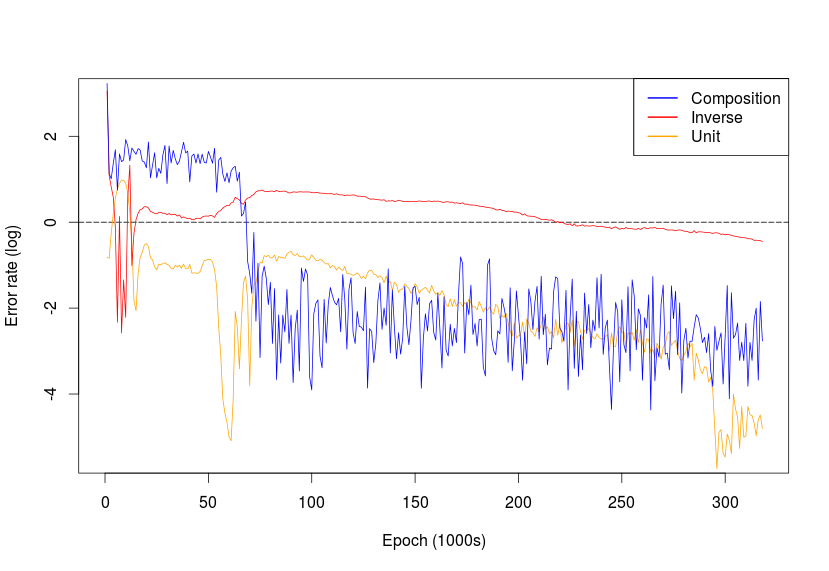
\includegraphics[width=\linewidth]{../img/z10_90percent.png}
\end{figure}
\begin{figure}[h]
\centering
\caption{Different values of "half" found during different runs. The first run (red) was very peculiar since it had over 2 700 000 epochs, but this representation settled already around epoch 300 000. It is not clear how this interacts with the rest of the elements.}
\label{table:z10_half}
\begin{tabular}{|c|c|c|c|c|c|}
\hline
\textcolor{red}{-0.9417969} & \textcolor{blue}{5.5017343} & \textcolor{blue}{5.500125} & 0.5014977 & \textcolor{blue}{5.500004} & \textcolor{blue}{5.507943}\\
\hline
\end{tabular}
\end{figure}

\begin{figure}[h]
\centering
\caption{Extension groups generated in two runs (read left to right, top to bottom). The blue elements are supposed to be in the original embedding, i.e. they should be 1...9 ascending with the last 3 elements being 0, "half", 1 respectively. In the first run we see that we have had very low success, even though the first half+half looks promising. The second run had much better success and with the exception of 9 it hit all original elements reasonably well, even those last 3.}
\label{table:z10_half_generator}
\begin{tabular}{ccccc}
\textbf{5.500004} & \textcolor{blue}{0.99998194} & 10.919293 & \textcolor{blue}{6.419118} & 1.9191066\\
 \textcolor{blue}{9.268123} & 4.7680063 & \textcolor{blue}{0.26805452} & 12.234171 & \textcolor{blue}{7.7339497}\\
3.2338893 & \textcolor{blue}{8.733828} & 4.233731 & \textcolor{blue}{1.9053116} & 9.292908 \\
\textcolor{blue}{4.792793} & 0.2928396 & \textcolor{blue}{12.189646} & 7.6894255 & \textcolor{blue}{3.1893663}\\
\textbf{8.689303} & \textcolor{blue}{4.189211}\\
 \\
\hline\\

\textbf{5.5069175} & \textcolor{blue}{0.99456155} & 6.5232387 & \textcolor{blue}{2.0135} & 7.5396843\\
\textcolor{blue}{3.032562} & 8.556266 & \textcolor{blue}{4.051762} & 3.872835 & \textcolor{blue}{5.4972463}\\
0.9848655 & \textcolor{blue}{6.5135655} & 2.0038028 & \textcolor{blue}{7.530016} & 3.022867\\
\textcolor{blue}{8.546589} & 4.04206 & \textcolor{blue}{3.9609222} & 4.6975384 & \textcolor{blue}{0.18309715}\\
\textbf{5.713754} & \textcolor{blue}{1.20193}
\end{tabular}

\end{figure}


\subsection{$\mathbb{Z}_{20}$}
The second group we experimented with was $\mathbb{Z}_{20}$. Because of its larger size, the experiments with it were longer. 

Once again, the equation by which we extend the group was $a+a=1$. The results of one experiment can be seen in \Autoref{graph:z20_90percent}. Once again, $10\%$ was excluded from the training. The trend lines are similar to $\mathbb{Z}_{10}$ (\Autoref{graph:z10_90percent}), with composition and inverse training quickly, while inverse lags behind. The inverse line is much noisier, because now the testing data has 2 elements, out of which 5 are chosen for testing (with repetition).

Values for the half in different runs can be seen in \Autoref{table:z20_half}. Once again, the algorithm usually found one of the two intuitive answers, 0.5 and 10.5. A graph showing the iterated composition of the half is depicted in \Autoref{graph:z20_half_generator}. As we see, the learned structure appears at first as very similar to the expected $\mathbb{Z}_{40}$, however we start seeing very large deviation after 40 compositions. The cause of this is unknown, but we suspect it could be caused by the network not learning the associativity axiom. Indeed, $19+1\doteq$19+(half+half) outputs correctly $0$, however (19+half)+half does not output 0.

\begin{figure}[h]
\centering
\caption{A $\mathbb{Z}_{20}$ learning run. We see that the trends we observed in $\mathbb{Z}_{10}$ continue, and it appears that extra time is not needed. However, in different runs we encountered difficulties with learning the inverse function.}
\label{graph:z20_90percent}
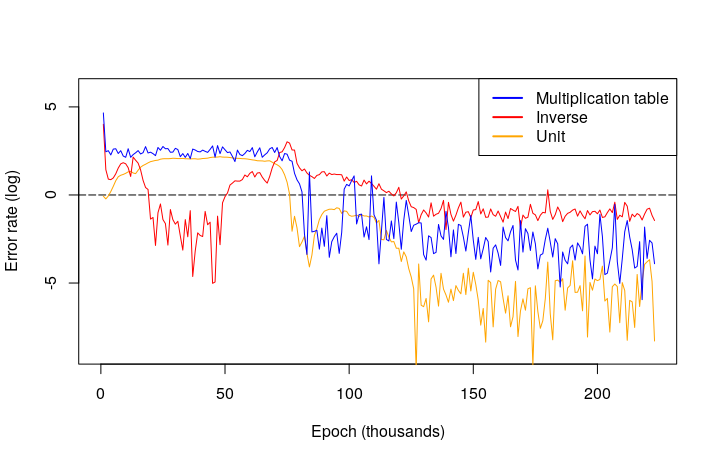
\includegraphics[width=\linewidth]{../img/z20_90percent.png}
\end{figure}

\begin{figure}[h]
\centering
\caption{Values for the half in different $\mathbb{Z}_{20}$ runs. Once again, the reason for why the red one is so different is unknown. The tendency towards 0.5 instead of 10.5 can be attributed to the fact that the initial parameters have been restricted to avoid overflow errors.}
\label{table:z20_half}
\begin{tabular}{|c|c|c|c|c|}
\hline
0.4999506 & \textcolor{red}{-6.5685954} & \textcolor{blue}{10.500707} & 0.49987993 & 0.5000777\\
\hline
0.49967808 & 0.49978873 & 0.49993014 & 0.50047106 & \textcolor{blue}{10.499506}\\
\hline
\end{tabular}
\end{figure}

\begin{figure}[h]
\centering
\caption{An example of a group generated from the "half" element. We see that there were no problems with addition of the half, except the modulus is not applied correctly.}
\label{graph:z20_half_generator}
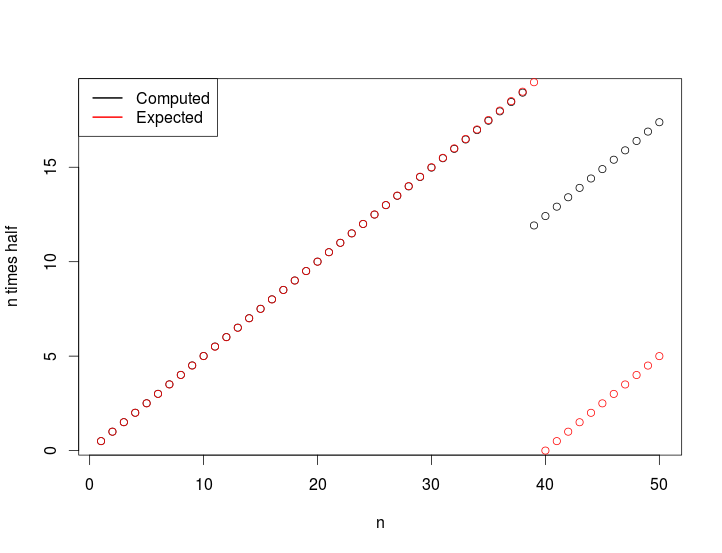
\includegraphics[width=0.8\linewidth]{../img/z20_half_plot.png}
\end{figure}

\subsection{Infinite group $\mathbb{Z}$}

The last cyclic group experiment was with the infinite group $(\mathbb{Z},+)$. The training set comprised of integers from an interval $[-10000,10000]$ in order to avoid overflow errors. Because neural network learning is already hard on such a diverse set, we opted to not exclude any data for training. 

$a+a=1$ still has no solution in this group. In contrast to the previous cases, there is only one intuitive solution and that is $\frac{1}{2}$. The group generated by this $\frac{1}{2}$ is isomorphic to the original. Unfortunately, we were unable to get to this point. The learned half was 
-1.1713637. When we tried to generate some elements of the extension, we obtained

\begin{tabular}{cccccc}
1&2&3&4&5&6\\
\hline
-1.1713637&1.0000439&2.2069557&2.8777812&3.2506382&3.4578807\\
 \\
7&8&9&10\\
\hline 
3.57307&3.637094&3.6726806&3.6924593
\end{tabular}

Indeed, the learned half+half=1, but the composition fails for larger iterations.
\begin{figure}
\caption{$\mathbb{Z}$ as an infinite group. Because of limitations of the software, we only trained on the interval $[-10000,10000]$ (hence the trained group is not really infinite). There was no testing set, but the network seemed to generalize well even outside of the training interval. Examples are computed $11000^{-1}=-11001.614$ or $15000+(-12000)=2999.9941$.}
\centering
\label{graph:z_inf}
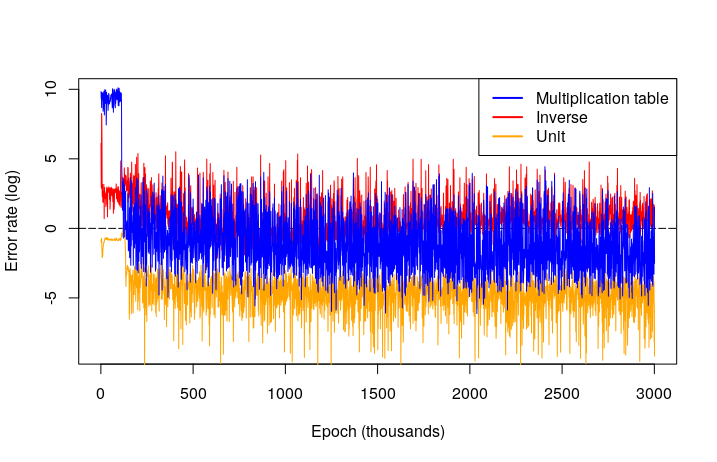
\includegraphics[width=\linewidth]{../img/z_inf.png}
\end{figure}

\section{Symmetric groups}
Symmetric groups, or permutation groups are the most complex finite groups. Indeed, a corollary from Cayley's theorem  is that every finite group is isomorphic to a symmetric group of large enough size (\cite{cayley}). This is why they have been chosen for further experiments.

Every symmetric group is generated by the set of transpositions of two elements. Each element can therefore be written as a sequence of transpositions. Although this sequence is not unique, all such sequences have the same length. For each permutation $\sigma$ we define $\text{sgn}(\sigma)=(-1)^l$ where $l$ is this number of transpositions. It also holds that $\text{sgn}(\sigma_1\circ\sigma_2)=\text{sgn}(\sigma_1)\text{sgn}(\sigma_2)$. Therefore $\text{sgn}(\sigma\circ\sigma)=1$. (proofs in \cite{Lingebra})

For this reason the equation that we sought to find the extension for is $h\circ h=(0,1)$ where $(0,1)$ denotes the transposition of elements $0$ and $1$. $\text{sgn}((0,1))=-1$, therefore we know that $h$ can not be in the original group. 

The structure of this extension is suspected to be some form of the semidirect product of $S_n\times\mathbb{Z}_2$, although the basic semidirect product appears to be insufficient.

\subsection{$S_4$ with a basic grounding}

$S_4$ is the group of permutations of 4 elements. A "na\"{i}ve" grounding of elements was chosen first. It assigns each permutation $(a,b,c,d)$\footnote{This being the full representation of the permutation.} the element $[a,b,c,d]\in\mathbb{R}^4$. The advantage of this grounding is its simplicity and shortness. The main disadvantage, however, is that the mean squared error loss function is biased. We can see this on an example where $[0,1,2,3]$ is one transposition away from both $[1,0,2,3]$ and $[3,1,2,0]$, however in the latter case the mean squared error is considerably higher. 

For the training we once again use only 90\% of the data. During the training we expectedly observe significantly higher training times, as exemplified in \Autoref{graph:s4_basic}. This is also compounded by having slightly more elements (24). We are also unable to achieve the same precision. Learning of the unit was again very precise, see table \ref{table:s4_unit_basic}.

When it comes to learning of $h$, we see even more problems than in the case of cyclic groups. Some half elements are seen in table \ref{table:s4_half_basic}. They are noticeably different from each other, something we did not observe before. The reason why these were the vectors found is unknown. 

However, as we see in table \ref{table:s4_half_basic_gen}, generating even a small subgroup results in a failure. Since $h\circ h=(0,1)$, we expect that $h^4=(h\circ h)\circ(h\circ h)=(0,1)\circ(0,1)=e$. Unfortunately, we were never able to get this equation to hold with $h\circ(h\circ(h\circ h))))$. Once again, reason for this is unknown. But because $(h\circ h)\circ (h\circ h)$ yielded reasonable results, we suspect that again the associativity is the problem.

\begin{figure}
\caption{One run of learning the $S_4$ with the basic grounding. We see that the training is expectedly much slower than in the cyclic groups.}
\label{graph:s4_basic}
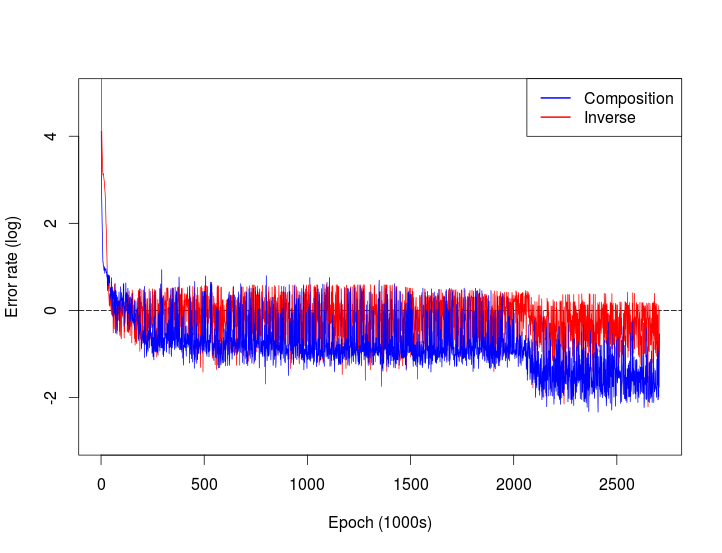
\includegraphics[width=0.9\linewidth]{../img/s4_comp+inv.png}
\end{figure}

\begin{figure}
\center
\caption{Units learned in $S_4$ with basic grounding. The expected output was $[0,1,2,3]$. As we see, they are very precise.}
\label{table:s4_unit_basic}
\begin{tabular}{l|cccc}
1.) &0.03967234 & 1.0745986 & 1.957876 & 2.9761093\\
\hline
2.) &0.00685234 & 1.0557759 & 2.1151063 & 3.2438033\\
\hline
3.) &0.01609807 & 0.9784863 & 2.011951 & 3.0008512\\
\end{tabular}
\end{figure}

\begin{figure}
\center
\caption{$h$-s found in several runs. As expected, they do not look like anything.}
\label{table:s4_half_basic}
\begin{tabular}{l|cccc}
1.)&-0.9288303 & 1.8216157 & 0.17884427 & 2.0224957\\
\hline
2.)&1.2200519 & 0.5469334 & 3.7773933 & -0.22675751\\
 \hline
3.)&2.9790108 & 2.5041845 & 1.9638568 & -1.186425\\
\end{tabular}
\end{figure}

\begin{figure}
\center
\caption{$h$ composed with itself several times. $h^2$ and $h^6$ should both be $[1,0,2,3]$. $h^4$ should be $[0,1,2,3]$.}
\label{table:s4_half_basic_gen}
\begin{tabular}{c|cccc}
$h$   & 2.9790108 & 2.5041845 & 1.9638568 & -1.186425\\
$h^2$ & 1.0137038 & 0.6440371 & 1.960084 & 3.0298772\\
$h^3$ & 1.899735 & 0.6546894 & 2.3109381 & 2.1213117\\
$h^4$ & 1.4959755 & 0.52787334 & 2.564281 & 2.4759564\\
$h^5$ & 1.3819728 & 0.7297171 & 2.8694618 & 2.1578472\\
$h^6$ & 1.1029358 & 0.97653824 & 3.1764572 & 1.9179444\\

\end{tabular}
\end{figure}

\subsection{$S_4$ with matrix grounding}
To fix the problem with the bias of the loss function we add the "one-of-n" representation. This representation is used for elements that are equally different from each other. This representation attaches to each of the $n$ elements a vector from the canonical basis of $\mathbb{R}^n$. If we take the basic representation of $S_4$ and change every element to its one-of-n representation, we get a vector in $\mathbb{R}^{16}$ that has exactly four ones and the rest are zeroes. For example 
$$(1,2,0,3)\rightarrow \left((0,1,0,0),(0,0,1,0),(1,0,0,0),(0,0,0,1)\right)$$

This erases the loss function bias, because now the mean squared difference between any two permutations depends only on the number of elements switched. One-to-n representation can also be seen as the matrix representation. Indeed, $(1,2,0,3)$ can be represented as
$$
\left(
\begin{matrix}
0 & 1 & 0 & 0\\
0 & 0 & 1 & 0\\
1 & 0 & 0 & 0\\
0 & 0 & 0 & 1
\end{matrix}
\right)
\left(
\begin{matrix}
a\\
b\\
c\\
d
\end{matrix}
\right)
=
\left(
\begin{matrix}
b\\
c\\
a\\
d
\end{matrix}
\right).
$$

A proof of this is an easy exercise in linear algebra. \\

This new grounding, however, brought several new problems. For example $3/4$-ths of the expected output are zeroes. This created a problem early on in the experimentation with the network only outputting a zero vector on any input. That is the reason why leaky ReLU had been used as an activation function as opposed to standard ReLU. This change solved this problem, since they avoid the "neuron death" - a situation where input to ReLU is so negative that it always outputs 0 and thus has no gradient.

Another problem was the size of the vectors relative to the number of elements, e.g. $S_3$ has only 6 elements but this representation has size 9. However, since the size of the group $S_n$ grows exponentially while the matrix representation only quadraticaly, for large enough $n$ the benefits of a less biased loss function outweigh the costs. Unfortunately, because of the amount of computation power needed to get to this point we were not able to verify this hypothesis.\\

As we can see in \Autoref{graph:s4_matrix}, this representation is still  efficient for composition, but the inverse is clearly wrong. Furthermore, as we see in table \ref{table:s4_matrix_unit}, the unit was usually significantly different from what was expected. This is the place where a penalty for straying away from an element could help significantly, as this problem most likely emerged as a consequence of the increase in dimension.

These two factors lead to the consequence that the inverse is not able to output elements of the grounding. If it did, composition would also output $a^{-1}a$ in grounding, but the learned $e$ is not in it.\\

The extension element $h$ is shown in table \ref{table:s4_matrix_half} along with parts of the generated subgroup. In the same vein as before, $h\circ h$ shows promise, but $h^4$ breaks down.

\begin{figure}
\center
\caption{$S_4$ with matrix grounding. The composition is very successful, but the inverse is not.}
\label{graph:s4_matrix}
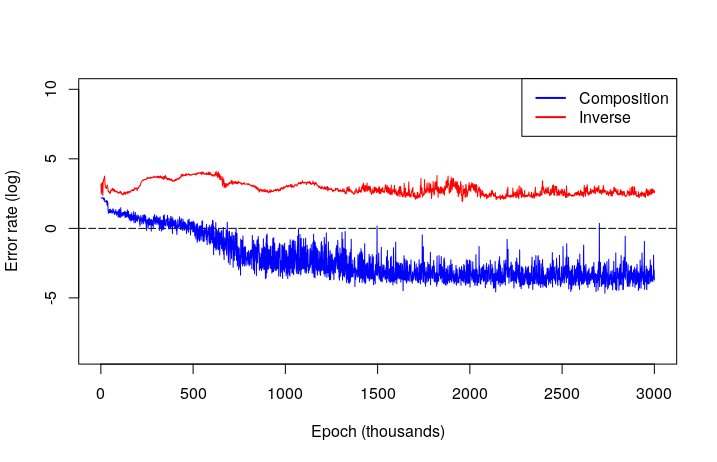
\includegraphics[width=\linewidth]{../img/s4_matrix.png}
\end{figure}

\begin{figure}
\center
\caption{Units found in $S_4$ with matrix representation. An identity matrix was expected. Places where 1 was expected are blue, black ones are for 0.}
\label{table:s4_matrix_unit}
\begin{tabular}{cccc}
\textcolor{blue}{0.9291287} & 0.39432997 & -0.09073094 & -0.00462165\\
-0.49930313 & \textcolor{blue}{2.5813785} & -1.0001388 & -0.51179993\\
0.38528794 & 0.32126167 & \textcolor{blue}{1.4879085} & -0.3122037\\
0.16110185 & -0.10436057 & -0.3780875 & \textcolor{blue}{1.356762}\\
 \\
\hline
\\
 \textcolor{blue}{0.36581007} & 0.11518399 & -0.29025748  & 0.7275856\\
0.38638538 & \textcolor{blue}{0.95944846} & -0.47597495 & -0.14604506\\
0.203323 & -0.15147878 & \textcolor{blue}{0.65808797} & -0.03862157\\
0.4341608 & -0.57306635 & -0.15940993 & \textcolor{blue}{1.5463064}
\end{tabular}
\end{figure}

\begin{figure}
\center
\caption{An extension attempt for $S_4$ with matrix representation. The blue numbers are expected to be $1$ and black ones $0$. As we see, $h^2$ is pretty much exactly what we wanted, but $h^4$ breaks down.}
\label{table:s4_matrix_half}
\begin{tabular}{lcccc}

$h$&-0.44275028 & 0.45813385 & 0.84849375 & -0.4929848\\
 &0.29338264 & 0.25557452 & 0.701611 & -0.33617198\\
 &0.5497755 & 0.75910103 & -0.16280994 & -0.17575327\\
 &0.20515643 & 0.25966993 & 0.10358979 & 1.0272595\\
 
 \hline
 
$h\circ h$&0.0016880417 & \textcolor{blue}{0.99703968} & -0.0002135747 & -0.0009868203\\
 &\textcolor{blue}{0.99901026} & -0.0018832732 & -0.0010174632 & 0.0011361403\\
 &-0.0027710588 & -0.0013556076 & \textcolor{blue}{1.0073379} & -0.001112761\\
 &-0.0005431428 & 0.0049326816 & -0.0010595275 & \textcolor{blue}{1.00323}\\
 
 \hline
 
 $h^4$&\textcolor{blue}{0.72058374} & 0.17218184	& 0.04241377 & 0.04261543\\
&0.4558762 & \textcolor{blue}{-0.00405501}	& 0.55539876 & 0.00293861\\
&-0.02832983 & 0.10163078 & \textcolor{blue}{0.4973646} & 0.4502491\\
&-0.02180864 & 0.6911213	& -0.02542126 &	\textcolor{blue}{0.4643306}

\end{tabular}

\end{figure}

\chapter*{Conclusion}
\addcontentsline{toc}{chapter}{Conclusion}
We have seen some promising results with regards to using neural networks to simulate particular mathematical models by learning on propositions that are true/false in them. We have successfully learned neural representations of groups, namely the cyclic and symmetric groups. Another focus of the work was building extensions to those models, relying on the learned functions.\\

For every model built here we used the multiplication table to learn the composition operation. Even despite the fact that the whole table is not needed (we have had good results even with 10\% of the table missing), prior knowledge of the structure is still required. In order to truly follow the ideas of the model theory, we would need to drop the table altogether. How to do this is currently not known and would be a subject to further experimentation.\\

Another place to improve the method shown here is the grounding, specifically the usage of handpicked representations. This would ideally also be eliminated, since it is another essential part of the model that relies on prior knowledge of the structures. For the self-finding of the groundings we could use recurrent neural networks, which are widely used for feature extraction. Another method that could improve performance is mutable grounding, i.e. grounding that could change during the learning process to better reflect the structure learned. However, this might be quite nontrivial.\\

A very large part of this thesis is model extension. Despite initial optimism stemming from the successes of the finite cyclic groups, the results have been rather lackluster. We speculate that this is caused by the fact that we used the multiplication table rather than the associativity axiom. The associativity obviously holds in the original universe, since the multiplication table had been learned quite efficiently. One way to ensure associativity on the extension as well would be introduction of axioms such as $(h\cdot a)\cdot b = h\cdot (a\cdot b)$ where $h$ is the extension element. However, training for general associativity - i.e. associativity on the whole domain $\mathbb{R}^n$ might slow down the learning process severely.\\

Because the work shown here is very early, there was little focus on the end goal - building an oracle that would gauge the probability that a given sentence is true. This would be a boon to the automated theorem proving community. Current trend is to use machine learning on the sentences themselves, thus skipping the models altogether. This approach has considerable limitations.

Unfortunately, the model-building process is very slow (order of hours on a home computer), therefore building an array of models for every problem would take some time. Classical Automated theorem proving competitions run in relatively short times (minutes), rendering this method rather unwieldy for usage in the state it is in right now. There is however a feasible niche for this model-based oracle in recent large-theory competitions and benchmarks and in theory building, i.e. expanding a given theory without a set goal. Large-theory benchmarks such as CASC LTB and the MPTP Challenge provide a large global time limit (days) for solving many related
problems. Machine learning of useful models for predicting the
validity of lemmas and conjectures could be very useful there.

Another area where the neural models could be useful is axiom selection, like SRASS described in \cite{model_axiom_selection}. Proving a conjecture $C$ from a large knowledge base usually needs only a subset of the axioms. Since automated theorem provers perform better on smaller axiom sets, finding such a subset is crucial. SRASS attempts this by numbering the axioms in the knowledge base $\varphi_1,\varphi_2,\dots$ and then finding a model for $\{\neg C,\varphi_1,\dots \varphi_n\}$ for ever larger $n$. If no such model exists, $\varphi_1,\dots \varphi_n$ is the desired subset on which the theorem prover can run.

%%% Bibliography
%%% Bibliography (literature used as a source)
%%%
%%% We employ bibTeX to construct the bibliography. It processes
%%% citations in the text (e.g., the \cite{...} macro) and looks up
%%% relevant entries in the bibliography.bib file.
%%%
%%% The \bibliographystyle command selects, which style will be used
%%% for references from the text. The argument in curly brackets is
%%% the name of the corresponding style file (*.bst). Both styles
%%% mentioned in this template are included in LaTeX distributions.

\bibliographystyle{plainnat}    %% Author (year)
% \bibliographystyle{unsrt}     %% [number]

\renewcommand{\bibname}{Bibliography}

%%% Generate the bibliography. Beware that if you cited no works,
%%% the empty list will be omitted completely.

\bibliography{bibliography}

%%% If case you prefer to write the bibliography manually (without bibTeX),
%%% you can use the following. Please follow the ISO 690 standard and
%%% citation conventions of your field of research.

% \begin{thebibliography}{99}
%
% \bibitem{lamport94}
%   {\sc Lamport,} Leslie.
%   \emph{\LaTeX: A Document Preparation System}.
%   2nd edition.
%   Massachusetts: Addison Wesley, 1994.
%   ISBN 0-201-52983-1.
%
% \end{thebibliography}


%%% Figures used in the thesis (consider if this is needed)
%\listoffigures

%%% Tables used in the thesis (consider if this is needed)
%%% In mathematical theses, it could be better to move the list of tables to the beginning of the thesis.
%\listoftables

%%% Abbreviations used in the thesis, if any, including their explanation
%%% In mathematical theses, it could be better to move the list of abbreviations to the beginning of the thesis.
%\chapwithtoc{List of Abbreviations}

%%% Attachments to the master thesis, if any. Each attachment must be
%%% referred to at least once from the text of the thesis. Attachments
%%% are numbered.
%%%
%%% The printed version should preferably contain attachments, which can be
%%% read (additional tables and charts, supplementary text, examples of
%%% program output, etc.). The electronic version is more suited for attachments
%%% which will likely be used in an electronic form rather than read (program
%%% source code, data files, interactive charts, etc.). Electronic attachments
%%% should be uploaded to SIS and optionally also included in the thesis on a~CD/DVD.
%%% Allowed file formats are specified in provision of the rector no. 72/2017.
%\appendix
%\chapter{Attachments}

%\section{First Attachment}

\openright
\end{document}
